% Options for packages loaded elsewhere
% Options for packages loaded elsewhere
\PassOptionsToPackage{unicode}{hyperref}
\PassOptionsToPackage{hyphens}{url}
%
\documentclass[
  letterpaper,
]{book}
\usepackage{xcolor}
\usepackage{amsmath,amssymb}
\setcounter{secnumdepth}{5}
\usepackage{iftex}
\ifPDFTeX
  \usepackage[T1]{fontenc}
  \usepackage[utf8]{inputenc}
  \usepackage{textcomp} % provide euro and other symbols
\else % if luatex or xetex
  \usepackage{unicode-math} % this also loads fontspec
  \defaultfontfeatures{Scale=MatchLowercase}
  \defaultfontfeatures[\rmfamily]{Ligatures=TeX,Scale=1}
\fi
\usepackage{lmodern}
\ifPDFTeX\else
  % xetex/luatex font selection
\fi
% Use upquote if available, for straight quotes in verbatim environments
\IfFileExists{upquote.sty}{\usepackage{upquote}}{}
\IfFileExists{microtype.sty}{% use microtype if available
  \usepackage[]{microtype}
  \UseMicrotypeSet[protrusion]{basicmath} % disable protrusion for tt fonts
}{}
\makeatletter
\@ifundefined{KOMAClassName}{% if non-KOMA class
  \IfFileExists{parskip.sty}{%
    \usepackage{parskip}
  }{% else
    \setlength{\parindent}{0pt}
    \setlength{\parskip}{6pt plus 2pt minus 1pt}}
}{% if KOMA class
  \KOMAoptions{parskip=half}}
\makeatother
% Make \paragraph and \subparagraph free-standing
\makeatletter
\ifx\paragraph\undefined\else
  \let\oldparagraph\paragraph
  \renewcommand{\paragraph}{
    \@ifstar
      \xxxParagraphStar
      \xxxParagraphNoStar
  }
  \newcommand{\xxxParagraphStar}[1]{\oldparagraph*{#1}\mbox{}}
  \newcommand{\xxxParagraphNoStar}[1]{\oldparagraph{#1}\mbox{}}
\fi
\ifx\subparagraph\undefined\else
  \let\oldsubparagraph\subparagraph
  \renewcommand{\subparagraph}{
    \@ifstar
      \xxxSubParagraphStar
      \xxxSubParagraphNoStar
  }
  \newcommand{\xxxSubParagraphStar}[1]{\oldsubparagraph*{#1}\mbox{}}
  \newcommand{\xxxSubParagraphNoStar}[1]{\oldsubparagraph{#1}\mbox{}}
\fi
\makeatother

\usepackage{color}
\usepackage{fancyvrb}
\newcommand{\VerbBar}{|}
\newcommand{\VERB}{\Verb[commandchars=\\\{\}]}
\DefineVerbatimEnvironment{Highlighting}{Verbatim}{commandchars=\\\{\}}
% Add ',fontsize=\small' for more characters per line
\usepackage{framed}
\definecolor{shadecolor}{RGB}{241,243,245}
\newenvironment{Shaded}{\begin{snugshade}}{\end{snugshade}}
\newcommand{\AlertTok}[1]{\textcolor[rgb]{0.68,0.00,0.00}{#1}}
\newcommand{\AnnotationTok}[1]{\textcolor[rgb]{0.37,0.37,0.37}{#1}}
\newcommand{\AttributeTok}[1]{\textcolor[rgb]{0.40,0.45,0.13}{#1}}
\newcommand{\BaseNTok}[1]{\textcolor[rgb]{0.68,0.00,0.00}{#1}}
\newcommand{\BuiltInTok}[1]{\textcolor[rgb]{0.00,0.23,0.31}{#1}}
\newcommand{\CharTok}[1]{\textcolor[rgb]{0.13,0.47,0.30}{#1}}
\newcommand{\CommentTok}[1]{\textcolor[rgb]{0.37,0.37,0.37}{#1}}
\newcommand{\CommentVarTok}[1]{\textcolor[rgb]{0.37,0.37,0.37}{\textit{#1}}}
\newcommand{\ConstantTok}[1]{\textcolor[rgb]{0.56,0.35,0.01}{#1}}
\newcommand{\ControlFlowTok}[1]{\textcolor[rgb]{0.00,0.23,0.31}{\textbf{#1}}}
\newcommand{\DataTypeTok}[1]{\textcolor[rgb]{0.68,0.00,0.00}{#1}}
\newcommand{\DecValTok}[1]{\textcolor[rgb]{0.68,0.00,0.00}{#1}}
\newcommand{\DocumentationTok}[1]{\textcolor[rgb]{0.37,0.37,0.37}{\textit{#1}}}
\newcommand{\ErrorTok}[1]{\textcolor[rgb]{0.68,0.00,0.00}{#1}}
\newcommand{\ExtensionTok}[1]{\textcolor[rgb]{0.00,0.23,0.31}{#1}}
\newcommand{\FloatTok}[1]{\textcolor[rgb]{0.68,0.00,0.00}{#1}}
\newcommand{\FunctionTok}[1]{\textcolor[rgb]{0.28,0.35,0.67}{#1}}
\newcommand{\ImportTok}[1]{\textcolor[rgb]{0.00,0.46,0.62}{#1}}
\newcommand{\InformationTok}[1]{\textcolor[rgb]{0.37,0.37,0.37}{#1}}
\newcommand{\KeywordTok}[1]{\textcolor[rgb]{0.00,0.23,0.31}{\textbf{#1}}}
\newcommand{\NormalTok}[1]{\textcolor[rgb]{0.00,0.23,0.31}{#1}}
\newcommand{\OperatorTok}[1]{\textcolor[rgb]{0.37,0.37,0.37}{#1}}
\newcommand{\OtherTok}[1]{\textcolor[rgb]{0.00,0.23,0.31}{#1}}
\newcommand{\PreprocessorTok}[1]{\textcolor[rgb]{0.68,0.00,0.00}{#1}}
\newcommand{\RegionMarkerTok}[1]{\textcolor[rgb]{0.00,0.23,0.31}{#1}}
\newcommand{\SpecialCharTok}[1]{\textcolor[rgb]{0.37,0.37,0.37}{#1}}
\newcommand{\SpecialStringTok}[1]{\textcolor[rgb]{0.13,0.47,0.30}{#1}}
\newcommand{\StringTok}[1]{\textcolor[rgb]{0.13,0.47,0.30}{#1}}
\newcommand{\VariableTok}[1]{\textcolor[rgb]{0.07,0.07,0.07}{#1}}
\newcommand{\VerbatimStringTok}[1]{\textcolor[rgb]{0.13,0.47,0.30}{#1}}
\newcommand{\WarningTok}[1]{\textcolor[rgb]{0.37,0.37,0.37}{\textit{#1}}}

\usepackage{longtable,booktabs,array}
\usepackage{calc} % for calculating minipage widths
% Correct order of tables after \paragraph or \subparagraph
\usepackage{etoolbox}
\makeatletter
\patchcmd\longtable{\par}{\if@noskipsec\mbox{}\fi\par}{}{}
\makeatother
% Allow footnotes in longtable head/foot
\IfFileExists{footnotehyper.sty}{\usepackage{footnotehyper}}{\usepackage{footnote}}
\makesavenoteenv{longtable}
\usepackage{graphicx}
\makeatletter
\newsavebox\pandoc@box
\newcommand*\pandocbounded[1]{% scales image to fit in text height/width
  \sbox\pandoc@box{#1}%
  \Gscale@div\@tempa{\textheight}{\dimexpr\ht\pandoc@box+\dp\pandoc@box\relax}%
  \Gscale@div\@tempb{\linewidth}{\wd\pandoc@box}%
  \ifdim\@tempb\p@<\@tempa\p@\let\@tempa\@tempb\fi% select the smaller of both
  \ifdim\@tempa\p@<\p@\scalebox{\@tempa}{\usebox\pandoc@box}%
  \else\usebox{\pandoc@box}%
  \fi%
}
% Set default figure placement to htbp
\def\fps@figure{htbp}
\makeatother





\setlength{\emergencystretch}{3em} % prevent overfull lines

\providecommand{\tightlist}{%
  \setlength{\itemsep}{0pt}\setlength{\parskip}{0pt}}



 


\makeatletter
\@ifpackageloaded{tcolorbox}{}{\usepackage[skins,breakable]{tcolorbox}}
\@ifpackageloaded{fontawesome5}{}{\usepackage{fontawesome5}}
\definecolor{quarto-callout-color}{HTML}{909090}
\definecolor{quarto-callout-note-color}{HTML}{0758E5}
\definecolor{quarto-callout-important-color}{HTML}{CC1914}
\definecolor{quarto-callout-warning-color}{HTML}{EB9113}
\definecolor{quarto-callout-tip-color}{HTML}{00A047}
\definecolor{quarto-callout-caution-color}{HTML}{FC5300}
\definecolor{quarto-callout-color-frame}{HTML}{acacac}
\definecolor{quarto-callout-note-color-frame}{HTML}{4582ec}
\definecolor{quarto-callout-important-color-frame}{HTML}{d9534f}
\definecolor{quarto-callout-warning-color-frame}{HTML}{f0ad4e}
\definecolor{quarto-callout-tip-color-frame}{HTML}{02b875}
\definecolor{quarto-callout-caution-color-frame}{HTML}{fd7e14}
\makeatother
\makeatletter
\@ifpackageloaded{bookmark}{}{\usepackage{bookmark}}
\makeatother
\makeatletter
\@ifpackageloaded{caption}{}{\usepackage{caption}}
\AtBeginDocument{%
\ifdefined\contentsname
  \renewcommand*\contentsname{Table of contents}
\else
  \newcommand\contentsname{Table of contents}
\fi
\ifdefined\listfigurename
  \renewcommand*\listfigurename{List of Figures}
\else
  \newcommand\listfigurename{List of Figures}
\fi
\ifdefined\listtablename
  \renewcommand*\listtablename{List of Tables}
\else
  \newcommand\listtablename{List of Tables}
\fi
\ifdefined\figurename
  \renewcommand*\figurename{Figure}
\else
  \newcommand\figurename{Figure}
\fi
\ifdefined\tablename
  \renewcommand*\tablename{Table}
\else
  \newcommand\tablename{Table}
\fi
}
\@ifpackageloaded{float}{}{\usepackage{float}}
\floatstyle{ruled}
\@ifundefined{c@chapter}{\newfloat{codelisting}{h}{lop}}{\newfloat{codelisting}{h}{lop}[chapter]}
\floatname{codelisting}{Listing}
\newcommand*\listoflistings{\listof{codelisting}{List of Listings}}
\makeatother
\makeatletter
\makeatother
\makeatletter
\@ifpackageloaded{caption}{}{\usepackage{caption}}
\@ifpackageloaded{subcaption}{}{\usepackage{subcaption}}
\makeatother
\usepackage{bookmark}
\IfFileExists{xurl.sty}{\usepackage{xurl}}{} % add URL line breaks if available
\urlstyle{same}
\hypersetup{
  pdftitle={Numerical Methods for PDEs: An Interactive Journey},
  pdfauthor={Renu Dhadwal},
  hidelinks,
  pdfcreator={LaTeX via pandoc}}


\title{Numerical Methods for PDEs: An Interactive Journey}
\author{Renu Dhadwal}
\date{}
\begin{document}
\frontmatter
\maketitle

\renewcommand*\contentsname{Table of contents}
{
\setcounter{tocdepth}{2}
\tableofcontents
}

\mainmatter
\bookmarksetup{startatroot}

\chapter{Numerical Methods for PDEs: An Interactive
Journey}\label{numerical-methods-for-pdes-an-interactive-journey}

\bookmarksetup{startatroot}

\chapter{Welcome}\label{welcome}

Welcome to this interactive journey through \textbf{Numerical Methods
for Partial Differential Equations (PDEs)}.

You will explore the subject through \textbf{dialogues between Acharya
and Pavni}, discovering history, classification, and numerical methods
step by step.

\section{Levels}\label{levels}

\begin{itemize}
\tightlist
\item
  \href{chapters/level1_history_pdes.qmd}{Level 1: Origins of PDEs}
\item
  \href{chapters/Level2_classification_pdes.qmd}{Level 2: Classification
  of PDEs}
\item
  \href{chapters/level3_PDE_BCs.qmd}{Level 3: Physical Interpretation
  and boundary conditions}
\item
  \href{chapters/level4_finite_differences.qmd}{Level 4: Finite
  Difference Methods- Introduction with application to the Heat
  Eqaution}
\item
  \href{chapters/level5_Wave_Equation.qmd}{Level 5 : Hyperbolic PDEs}
\item
  \href{chapters/level6_von_neumann.qmd}{Level 6 : Von-Neumann Stability
  Analysis}
\end{itemize}

\begin{center}\rule{0.5\linewidth}{0.5pt}\end{center}

\bookmarksetup{startatroot}

\chapter{Stay tuned as new levels unlock --- from classification of PDEs
to discretization techniques and
beyond!}\label{stay-tuned-as-new-levels-unlock-from-classification-of-pdes-to-discretization-techniques-and-beyond}

\bookmarksetup{startatroot}

\chapter{Level 1: A Historical Glimpse of
PDEs}\label{level-1-a-historical-glimpse-of-pdes}

\textbf{Pavni:} Acharya, where did all these partial differential
equations come from? They seem so abstract.

\textbf{Acharya:} Ah, Pavni, they did not begin in abstraction. They
began with strings, heat, and the mysteries of the heavens.

\textbf{Pavni:} Strings? You mean music?

\textbf{Acharya:} Exactly! In 1746, \emph{d'Alembert} studied how a
vibrating string produces sound. From that, he wrote down the
\textbf{wave equation}. Soon after, \emph{Euler} extended it to drums
and membranes. So you see, music and mathematics are deeply connected.

\textbf{Pavni:} That's beautiful! And the heat equation?

\textbf{Acharya:} That came from \emph{Joseph Fourier} in the early
1800s. He asked: \emph{How does heat spread through a solid body?} His
answer was the \textbf{heat equation}, and in solving it he gave us the
gift of \textbf{Fourier series}.

\textbf{Pavni:} So Fourier series were born from studying heat?

\textbf{Acharya:} Precisely. And then \emph{Laplace} studied
gravitational attraction and derived the \textbf{Laplace equation},
describing potentials in physics. \emph{Poisson} later generalized it
with the \textbf{Poisson equation}, where sources appear inside the
field.

\textbf{Pavni:} So each new equation came from a real phenomenon.

\textbf{Acharya:} Just so. Later, in the 19th century, \emph{Navier} and
\emph{Stokes} wrote down the equations of fluid motion --- the
\textbf{Navier--Stokes equations}. Even today, their mysteries are not
fully solved.

\textbf{Pavni:} (smiling) So PDEs are not just formulas on paper. They
are echoes of sound, flows of heat, gravity, and water.

\textbf{Acharya:} Well said, Pavni. They are the language by which
nature speaks to us.

\bookmarksetup{startatroot}

\chapter{Level 2: Classification of
PDEs}\label{level-2-classification-of-pdes}

\textbf{Pavni:} Acharya, last time you told me how PDEs were born from
strings, heat, and flows. But there seem to be so many kinds of PDEs.
How do we organize them?

\textbf{Acharya:} A good question, Pavni. Mathematicians classify PDEs
in several ways, much like a botanist classifies plants. Let us begin
with the simplest.

\textbf{Pavni:} I am listening.

\textbf{Acharya:} First, by \textbf{order}. A PDE is first-order if the
highest derivative is first order, second-order if the highest is
second, and so on. For example, the transport equation
\(u_t + c u_x = 0\) is first-order, while the heat equation
\(u_t = \alpha u_{xx}\) is second-order.

\textbf{Pavni:} That part seems simple enough. What else?

\textbf{Acharya:} Next comes \textbf{linearity}. A PDE is linear if the
unknown function and its derivatives appear only linearly --- not
multiplied together, not inside a sine or square. The heat equation is
linear. But if you had a term like \(u u_x\), that would make it
nonlinear.

\textbf{Pavni:} So, nonlinear PDEs are trickier?

\textbf{Acharya:} Very much so! Nonlinearity makes life both harder and
richer.

\textbf{Pavni:} Are there other distinctions?

\textbf{Acharya:} Yes. Equations can be \textbf{homogeneous} or
\textbf{inhomogeneous} depending on whether the right-hand side is zero.
Laplace's equation is homogeneous, Poisson's equation is inhomogeneous.

\textbf{Acharya:} More generally, a non-homogeneous PDE can be written
as:\\
\[ F(t, x_1, x_2, \dots, x_n, u, u_t, u_{x_1}, \dots, u_{x_n}, u_{tt}, u_{x_1x_1}, \dots) = g(x_1, x_2, \dots, x_n, t), \]\\
where \(g\) is a nonzero source or forcing term. If \(g \equiv 0\), the
PDE is homogeneous.

\textbf{Pavni:} So the right-hand side introduces an external influence,
like heat sources or forces?

\textbf{Acharya:} Exactly. For example, \(u_{xx} + u_{yy} = f(x,y)\) is
the Poisson equation with a source term \(f(x,y)\). .

\textbf{Pavni:} I think I follow. But I have also heard words like
elliptic and hyperbolic. What do they mean?

\textbf{Acharya:} Ah, those arise for \textbf{second-order PDEs in two
variables}. Suppose we have:\\
\[ A u_{xx} + B u_{xy} + C u_{yy} + \dots = 0. \]\\
We look at the discriminant: \(B^2 - 4AC\).\\
- If it is less than 0, the PDE is \textbf{elliptic} (like Laplace's
equation).\\
- If it equals 0, the PDE is \textbf{parabolic} (like the heat
equation).\\
- If it is greater than 0, the PDE is \textbf{hyperbolic} (like the wave
equation).

\textbf{Pavni:} This reminds me of conic sections! Circles, parabolas,
and hyperbolas.

\textbf{Acharya:} Exactly. The analogy is deliberate --- both come from
the same quadratic form.

\textbf{Pavni:} And physically?

\textbf{Acharya:} Elliptic equations describe steady states --- like
equilibrium temperature distributions. Parabolic equations describe
diffusion, the smoothing of irregularities over time. Hyperbolic
equations describe wave-like motion, signals traveling with finite
speed.

\textbf{Pavni:} That helps me imagine them. So classification is not
just a game, but it tells us the nature of the solutions.

\textbf{Acharya:} Well said, Pavni. And it also guides how we design
numerical methods. An elliptic problem requires different strategies
than a hyperbolic one.

\textbf{Pavni:} Then I am eager to learn those strategies!

\textbf{Acharya:} Patience, Pavni. First we must prepare the ground.
Classification is the map; numerical methods are the journey.

\begin{center}\rule{0.5\linewidth}{0.5pt}\end{center}

\section{Mini Quizzes}\label{mini-quizzes}

\textbf{Quiz 1:} Identify the order\\
Which of the following is a second-order PDE?\\
1. \$ u\_t + cu\_x = 0 \$\\
2. \$ u\_t = \alpha u\_\{xx\} \$\\
3. \$ u u\_x = 0 \$

\begin{tcolorbox}[enhanced jigsaw, toprule=.15mm, opacityback=0, rightrule=.15mm, breakable, colframe=quarto-callout-tip-color-frame, coltitle=black, toptitle=1mm, titlerule=0mm, left=2mm, bottomrule=.15mm, leftrule=.75mm, colback=white, colbacktitle=quarto-callout-tip-color!10!white, bottomtitle=1mm, opacitybacktitle=0.6, title=\textcolor{quarto-callout-tip-color}{\faLightbulb}\hspace{0.5em}{Answer 1}, arc=.35mm]

Equation (2) \$ u\_t = \alpha u\_\{xx\} \$ is second-order because of
the \(u_{xx}\) term.

\end{tcolorbox}

\begin{center}\rule{0.5\linewidth}{0.5pt}\end{center}

\textbf{Quiz 2:} Linearity check\\
Which PDE is nonlinear?\\
1. \$ u\_t = \alpha u\_\{xx\} \$\\
2. \$ u\_t + u u\_x = 0 \$

\begin{tcolorbox}[enhanced jigsaw, toprule=.15mm, opacityback=0, rightrule=.15mm, breakable, colframe=quarto-callout-tip-color-frame, coltitle=black, toptitle=1mm, titlerule=0mm, left=2mm, bottomrule=.15mm, leftrule=.75mm, colback=white, colbacktitle=quarto-callout-tip-color!10!white, bottomtitle=1mm, opacitybacktitle=0.6, title=\textcolor{quarto-callout-tip-color}{\faLightbulb}\hspace{0.5em}{Answer 2}, arc=.35mm]

Equation (2) is nonlinear because of the product term \(u u_x\).

\end{tcolorbox}

\begin{center}\rule{0.5\linewidth}{0.5pt}\end{center}

\textbf{Quiz 3:} Homogeneous or inhomogeneous\\
Classify: \$ u\_\{xx\} + u\_\{yy\} = f(x,y) \$.

\begin{tcolorbox}[enhanced jigsaw, toprule=.15mm, opacityback=0, rightrule=.15mm, breakable, colframe=quarto-callout-tip-color-frame, coltitle=black, toptitle=1mm, titlerule=0mm, left=2mm, bottomrule=.15mm, leftrule=.75mm, colback=white, colbacktitle=quarto-callout-tip-color!10!white, bottomtitle=1mm, opacitybacktitle=0.6, title=\textcolor{quarto-callout-tip-color}{\faLightbulb}\hspace{0.5em}{Answer 3}, arc=.35mm]

It is \textbf{inhomogeneous}, since the right-hand side is not zero.

\end{tcolorbox}

\begin{center}\rule{0.5\linewidth}{0.5pt}\end{center}

\textbf{Quiz 4:} Type of second-order PDE\\
For \$ u\_\{xx\} + 2u\_\{xy\} + u\_\{yy\} = 0 \$, compute \$ B\^{}2 -
4AC \$. What type is it?

\begin{tcolorbox}[enhanced jigsaw, toprule=.15mm, opacityback=0, rightrule=.15mm, breakable, colframe=quarto-callout-tip-color-frame, coltitle=black, toptitle=1mm, titlerule=0mm, left=2mm, bottomrule=.15mm, leftrule=.75mm, colback=white, colbacktitle=quarto-callout-tip-color!10!white, bottomtitle=1mm, opacitybacktitle=0.6, title=\textcolor{quarto-callout-tip-color}{\faLightbulb}\hspace{0.5em}{Answer 4}, arc=.35mm]

Here, \(A = 1, B = 2, C = 1\).\\
\$ B\^{}2 - 4AC = 2\^{}2 - 4(1)(1) = 0 \$.\\
So it is \textbf{parabolic}.

\end{tcolorbox}

\begin{center}\rule{0.5\linewidth}{0.5pt}\end{center}

\textbf{Quiz 5:} Physical meaning\\
Match each equation with its physical interpretation:\\
- Heat equation\\
- Wave equation\\
- Laplace's equation

\begin{enumerate}
\def\labelenumi{(\alph{enumi})}
\tightlist
\item
  Steady state\\
\item
  Wave-like motion\\
\item
  Diffusion in time
\end{enumerate}

\begin{tcolorbox}[enhanced jigsaw, toprule=.15mm, opacityback=0, rightrule=.15mm, breakable, colframe=quarto-callout-tip-color-frame, coltitle=black, toptitle=1mm, titlerule=0mm, left=2mm, bottomrule=.15mm, leftrule=.75mm, colback=white, colbacktitle=quarto-callout-tip-color!10!white, bottomtitle=1mm, opacitybacktitle=0.6, title=\textcolor{quarto-callout-tip-color}{\faLightbulb}\hspace{0.5em}{Answer 5}, arc=.35mm]

\begin{itemize}
\tightlist
\item
  Heat equation → (c) Diffusion in time\\
\item
  Wave equation → (b) Wave-like motion\\
\item
  Laplace's equation → (a) Steady state\\
\end{itemize}

\end{tcolorbox}

\bookmarksetup{startatroot}

\chapter{Level 3: PDEs, their Physical Meaning, and Boundary
Conditions}\label{level-3-pdes-their-physical-meaning-and-boundary-conditions}

\textbf{Pavni:} Acharya, PDEs still feel mysterious. What do they
\emph{really} mean?

\textbf{Acharya:} Good question. PDEs describe how a quantity changes
with respect to \textbf{both time and space}. Think of:\\
- Heat spreading in a rod\\
- Waves traveling along a string\\
- Fluid flowing through a pipe

All of these involve rates of change in multiple directions, and that's
why PDEs come into play.

\textbf{Pavni:} So PDEs are the language of physics in extended domains?

\textbf{Acharya:} Exactly. But to make their solutions unique and
physically meaningful, we need \textbf{boundary conditions}. Let's
explore them one by one.

\begin{center}\rule{0.5\linewidth}{0.5pt}\end{center}

\section{Dirichlet Condition}\label{dirichlet-condition}

\textbf{Acharya:} Dirichlet means fixing the value of the solution at
the boundary.

\textbf{Pavni:} Like holding both ends of a rod at 100 °C?

\textbf{Acharya:} Precisely. It represents physical situations where the
boundary is controlled by an external source---like contact with a
thermostat.

\begin{center}\rule{0.5\linewidth}{0.5pt}\end{center}

\section{Neumann Condition}\label{neumann-condition}

\textbf{Acharya:} Neumann means fixing the derivative, often
representing \textbf{flux}.

\textbf{Pavni:} So in the rod, saying no heat flows out means the
temperature gradient at the end is zero?

\textbf{Acharya:} Exactly. That's an insulated boundary.

\begin{center}\rule{0.5\linewidth}{0.5pt}\end{center}

\section{Robin (Mixed) Condition}\label{robin-mixed-condition}

\textbf{Acharya:} Robin mixes the two:\\
\[
a u + b \frac{\partial u}{\partial n} = c.
\]

\textbf{Pavni:} Is that like when heat escapes to the air?

\textbf{Acharya:} Yes---convective cooling. The flux depends on both the
temperature at the boundary and the environment.

\begin{center}\rule{0.5\linewidth}{0.5pt}\end{center}

💡 Quick Recap

\begin{itemize}
\tightlist
\item
  \textbf{Dirichlet} → Value fixed (e.g., temperature = 100 °C).\\
\item
  \textbf{Neumann} → Flux fixed (e.g., insulated boundary).\\
\item
  \textbf{Robin} → Combination (e.g., convective heat loss).
\end{itemize}

\begin{center}\rule{0.5\linewidth}{0.5pt}\end{center}

\subsection{📝 Mini-Quiz}\label{mini-quiz}

\begin{enumerate}
\def\labelenumi{\arabic{enumi}.}
\tightlist
\item
  A vibrating string held fixed at both ends uses which boundary
  condition?\\

  Answer

  \textbf{Dirichlet.} The displacement of the string is zero at both
  ends.
\item
  If a wall is perfectly insulated, what type of boundary condition
  applies to temperature?\\

  Answer

  \textbf{Neumann.} The derivative (temperature gradient) is zero,
  meaning no heat flux.
\item
  Which boundary condition models cooling of hot coffee in a room?\\

  Answer

  \textbf{Robin.} Heat loss depends on both the coffee's surface
  temperature and the room temperature (convection).
\end{enumerate}

\begin{center}\rule{0.5\linewidth}{0.5pt}\end{center}

\textbf{Pavni:} Now I see it! PDEs tell the story inside the domain, and
boundary conditions set the rules at the edges.

\textbf{Acharya:} Well said. Together, they form the complete model of a
physical system.

\begin{center}\rule{0.5\linewidth}{0.5pt}\end{center}

\bookmarksetup{startatroot}

\chapter{Level 4: Finite Differences and the Heat
Equation}\label{level-4-finite-differences-and-the-heat-equation}

\textbf{Pavni:} Acharya, how do we actually \emph{approximate}
derivatives on a computer?

\textbf{Acharya:} We use the \textbf{finite difference method}. A
computer only works with discrete points, so we replace continuous
derivatives with \textbf{difference quotients} on a \textbf{grid}. These
come directly from the \textbf{Taylor series}, and because we truncate
the series, each formula comes with a predictable \textbf{error term}.

\textbf{Pavni:} Can you give me an example?

\textbf{Acharya:} Suppose we have points \(x_0, x_1, \dots, x_N\) with
spacing \(\Delta x\). Around a point \(x_i\), Taylor's theorem gives us
expansions for \(u(x_{i+1})\) and \(u(x_{i-1})\). By combining them, we
obtain difference formulas:

\begin{itemize}
\item
  \textbf{Forward difference} for the first derivative: \[
  u'(x_i) = \frac{u(x_{i+1}) - u(x_i)}{\Delta x} - \tfrac{1}{2}u''(\xi)\,\Delta x,
  \] so the truncation error is \(\mathcal{O}(\Delta x)\).
\item
  \textbf{Backward difference}: \[
  u'(x_i) = \frac{u(x_i) - u(x_{i-1})}{\Delta x} + \tfrac{1}{2}u''(\xi)\,\Delta x,
  \] also error \(\mathcal{O}(\Delta x)\).
\item
  \textbf{Central difference}: \[
  u'(x_i) = \frac{u(x_{i+1}) - u(x_{i-1})}{2\Delta x} - \tfrac{1}{6}u^{(3)}(\xi)\,(\Delta x)^2,
  \] so the error is \(\mathcal{O}((\Delta x)^2)\) --- more accurate.
\item
  \textbf{Second derivative} (central difference): \[
  u''(x_i) = \frac{u(x_{i-1}) - 2u(x_i) + u(x_{i+1})}{(\Delta x)^2} - \tfrac{1}{12}u^{(4)}(\xi)\,(\Delta x)^2,
  \] with error \(\mathcal{O}((\Delta x)^2)\).
\end{itemize}

\textbf{Pavni:} So these formulas are not exact --- they always come
with an error term?

\textbf{Acharya:} Precisely. That error is called the \textbf{local
truncation error}. When we build numerical schemes for PDEs, these
errors accumulate step by step, and we'll have to balance them with
stability.

\textbf{Pavni:} I see. So finite differences give us algebraic formulas
for derivatives, but with a known accuracy.

\textbf{Acharya:} Exactly. That's the foundation of finite difference
methods.

\section{Application: The Heat
Equation}\label{application-the-heat-equation}

\textbf{Acharya:} Consider the 1D heat equation: \[
u_t = \alpha^2 u_{xx}^2, \quad 0 < x < 1,\; t>0
\] with boundary conditions \(u(0,t) = u(1,t) = 0\) and initial profile
\(u(x,0) = f(x)\).

We set up a grid: - In space: \(x_i = i\Delta x,\; i=0,\dots,N\)\\
- In time: \(t^n = n\Delta t,\; n=0,1,2,\dots\)

At each point, let \(u_i^n \approx u(x_i,t^n)\).

\textbf{Pavni:} And now we replace derivatives?

\textbf{Acharya:} Correct.\\
- Time derivative (forward difference): \[
  u_t(x_i,t^n) \approx \frac{u_i^{n+1} - u_i^n}{\Delta t}
  \] - Spatial second derivative (central difference): \[
  u_{xx}(x_i,t^n) \approx \frac{u_{i-1}^n - 2u_i^n + u_{i+1}^n}{(\Delta x)^2}
  \]

Plugging these into the PDE, we get: \[
\frac{u_i^{n+1} - u_i^n}{\Delta t} = \alpha^2 \,\frac{u_{i-1}^n - 2u_i^n + u_{i+1}^n}{(\Delta x)^2}.
\]

Rearranging: \[
u_i^{n+1} = u_i^n + \lambda\,(u_{i-1}^n - 2u_i^n + u_{i+1}^n),
\] where \(\lambda = \frac{\alpha^2 \Delta t}{(\Delta x)^2}\).

\begin{center}\rule{0.5\linewidth}{0.5pt}\end{center}

\section{Stability Condition}\label{stability-condition}

\textbf{Pavni:} So we can just keep applying this formula to march
forward in time?

\textbf{Acharya:} Yes, but with a caveat. This scheme, called
\textbf{FTCS (Forward Time, Central Space)}, is only stable if: \[
\lambda \leq \tfrac{1}{2}.
\]

\textbf{Pavni:} So if \(\Delta t\) is too large, the scheme fails?

\textbf{Acharya:} Exactly. The numerical solution will blow up, even
though the true solution is stable. Choosing \(\Delta t\) small enough
ensures stability.

\begin{tcolorbox}[enhanced jigsaw, toprule=.15mm, opacityback=0, rightrule=.15mm, breakable, colframe=quarto-callout-note-color-frame, coltitle=black, toptitle=1mm, titlerule=0mm, left=2mm, bottomrule=.15mm, leftrule=.75mm, colback=white, colbacktitle=quarto-callout-note-color!10!white, bottomtitle=1mm, opacitybacktitle=0.6, title=\textcolor{quarto-callout-note-color}{\faInfo}\hspace{0.5em}{Why the FTCS stability condition is \(\lambda \leq \tfrac{1}{2}\)}, arc=.35mm]

If the update is \[
u^{(n+1)} = A u^{(n)},
\] and the initial error is \(e^0\), then after \(n\) steps the error is
\[
e^{(n)} = A^n e^0.
\]

Using an induced matrix norm: \[
\|e^{(n)}\| = \|A^n e^0\| \;\le\; \|A^n\|\,\|e^0\|
\;\le\; \|A\|^n \|e^0\|.
\]

\begin{itemize}
\tightlist
\item
  If \(\|A\|\le 1\), the error never grows.\\
\item
  If \(\|A\|<1\), the error decays as \(n\to\infty\).\\
\item
  In general, the asymptotic condition is that the \textbf{spectral
  radius} \(\rho(A)<1\).
\end{itemize}

\begin{center}\rule{0.5\linewidth}{0.5pt}\end{center}

\subsubsection{Eigenvalues of the FTCS
matrix}\label{eigenvalues-of-the-ftcs-matrix}

For the FTCS tridiagonal matrix \(A\) (symmetric Toeplitz), the
eigenvalues are \[
\mu_k = 1 - 4 \lambda \,\sin^2\!\left(\frac{k\pi}{2(N-1)}\right), 
\qquad k=1,2,\dots,N-2,
\] where \(\lambda = \dfrac{\alpha^2 \Delta t}{(\Delta x)^2}\).

Thus the spectral radius is \[
\rho(A) = \max_{1\le k \le N-2} \big|\mu_k\big|
= \max_{1\le k \le N-2} \left|1 - 4r \sin^2\!\left(\tfrac{k\pi}{2(N-1)}\right)\right|.
\]

\begin{center}\rule{0.5\linewidth}{0.5pt}\end{center}

\subsubsection{Stability condition}\label{stability-condition-1}

\begin{itemize}
\tightlist
\item
  As \(N\to\infty\) (i.e.~\(\Delta x \to 0\)), the maximum of
  \(\sin^2(\cdot)\) tends to \(1\).\\
\item
  Therefore the most restrictive case is \[
  |1 - 4 \lambda| \le 1.
  \]
\item
  This simplifies to \[
  0 \;\le\; \lambda \;\le\; \tfrac{1}{2}.
  \]
\end{itemize}

\begin{center}\rule{0.5\linewidth}{0.5pt}\end{center}

✅ Thus, the \textbf{FTCS scheme is stable if and only if} \[
\lambda = \frac{\alpha \Delta t}{(\Delta x)^2} \;\le\; \tfrac{1}{2}.
\]

\end{tcolorbox}

\begin{center}\rule{0.5\linewidth}{0.5pt}\end{center}

\section{Mini-Quizzes}\label{mini-quizzes-1}

\textbf{Quiz 1:}\\
Let \(u(x) = x^2\). With \(\Delta x = 0.1\), approximate \(u'(1)\)
using:\\
1. Forward difference\\
2. Central difference

Compare with the exact derivative \(u'(1) = 2\). Which is more accurate?

\begin{tcolorbox}[enhanced jigsaw, toprule=.15mm, opacityback=0, rightrule=.15mm, breakable, colframe=quarto-callout-tip-color-frame, coltitle=black, toptitle=1mm, titlerule=0mm, left=2mm, bottomrule=.15mm, leftrule=.75mm, colback=white, colbacktitle=quarto-callout-tip-color!10!white, bottomtitle=1mm, opacitybacktitle=0.6, title=\textcolor{quarto-callout-tip-color}{\faLightbulb}\hspace{0.5em}{Answer 1}, arc=.35mm]

\begin{itemize}
\item
  Forward difference: \[
  \frac{u(1+\Delta x)-u(1)}{\Delta x}=\frac{(1.1)^2-1^2}{0.1}=\frac{1.21-1}{0.1}=2.1.
  \]
\item
  Central difference: \[
  \frac{u(1+\Delta x)-u(1-\Delta x)}{2\Delta x}
  =\frac{(1.1)^2-(0.9)^2}{0.2}=\frac{1.21-0.81}{0.2}=2.0.
  \]
\item
  Exact derivative: \(u'(1)=2\).
\end{itemize}

\textbf{Conclusion:} The central difference gives the exact value here
(error \(0\)), while the forward difference has error \(0.1\). Central
is more accurate (as expected --- it is second-order).

\end{tcolorbox}

\begin{center}\rule{0.5\linewidth}{0.5pt}\end{center}

\textbf{Quiz 2:}\\
Suppose \(\alpha = 1\), \(\Delta x = 0.1\). What is the maximum
\(\Delta t\) for stability in the explicit scheme?

(Hint:
\(\lambda = \dfrac{\alpha \Delta t}{(\Delta x)^2} \leq \tfrac{1}{2}\).)

\begin{tcolorbox}[enhanced jigsaw, toprule=.15mm, opacityback=0, rightrule=.15mm, breakable, colframe=quarto-callout-tip-color-frame, coltitle=black, toptitle=1mm, titlerule=0mm, left=2mm, bottomrule=.15mm, leftrule=.75mm, colback=white, colbacktitle=quarto-callout-tip-color!10!white, bottomtitle=1mm, opacitybacktitle=0.6, title=\textcolor{quarto-callout-tip-color}{\faLightbulb}\hspace{0.5em}{Answer 2}, arc=.35mm]

We need \[
\lambda=\frac{\alpha\,\Delta t}{(\Delta x)^2}\le\frac{1}{2}.
\] With \(\alpha=1\) and \(\Delta x=0.1\), \((\Delta x)^2=0.01\). So \[
\frac{\Delta t}{0.01}\le\frac{1}{2}\quad\Rightarrow\quad
\Delta t \le 0.01\times\frac{1}{2}=0.005.
\]

\textbf{Maximum allowable} \(\displaystyle \Delta t = 0.005\).

\end{tcolorbox}

\section{Heat equation --- Matrix Method with Non-zero Dirichlet
Conditions}\label{heat-equation-matrix-method-with-non-zero-dirichlet-conditions}

\textbf{Pavni:} We already saw how to discretize the heat equation with
FTCS. But can we write the whole scheme in a more compact way?

\textbf{Acharya:} Yes. That's where the \textbf{matrix method} comes in.
Let's recall the PDE: \[
u_t = \alpha^2 u_{xx}, \quad 0 < x < 1, \; t > 0,
\] with Dirichlet conditions \[
u(0,t) = L, \qquad u(1,t) = R,
\] and initial condition \(u(x,0)=f(x)\).

\textbf{Pavni:} So we still set up the grid in space and time?

\textbf{Acharya:} Exactly. The FTCS update at interior nodes is \[
u_i^{j+1} = u_i^j + \lambda \,(u_{i-1}^j - 2u_i^j + u_{i+1}^j),
\quad i=1,\dots,N_x-2,
\] where \(\lambda = \tfrac{\alpha^2 \Delta t}{\Delta x^2}\).

\textbf{Pavni:} That's a lot of coupled equations. How do we collect
them?

\textbf{Acharya:} We put all interior values into a vector \[
u^{(j)} =
\begin{bmatrix}
u_1^j \\
u_2^j \\
\vdots \\
u_{N_x-2}^j
\end{bmatrix}.
\]

\textbf{Pavni:} And the update rule becomes a matrix multiplication?

\textbf{Acharya:} Yes. We can write \[
u^{(j+1)} = A\,u^{(j)} + b,
\] where \(A\) is tridiagonal and \(b\) accounts for the boundary
conditions: \[
A =
\begin{bmatrix}
1-2\lambda & \lambda     &        &        &   \\
\lambda     & 1-2\lambda & \lambda      &        &   \\
      & \ddots & \ddots & \ddots &   \\
      &        & \lambda      & 1-2\lambda   & \lambda \\
      &        &        & \lambda      & 1-2\lambda
\end{bmatrix}, \qquad
b =
\begin{bmatrix}
\lambda L \\
0 \\
\vdots \\
0 \\
\lambda R
\end{bmatrix}.
\]

\textbf{Pavni:} So if \(L=R=0\), then \(b=0\) and we just have
\(u^{(j+1)} = A u^{(j)}\).

\textbf{Acharya:} Precisely. That's the beauty of the matrix method: it
organizes the scheme into a linear algebra update.

\begin{center}\rule{0.5\linewidth}{0.5pt}\end{center}

\subsection{Implementation in Python}\label{implementation-in-python}

Let us now implement the method in Python and compare with the exact
solution for \(f(x)=\sin(\pi x)\): \[
u(x,t) = e^{-\pi^2 \alpha t}\,\sin(\pi x).
\]

\pandocbounded{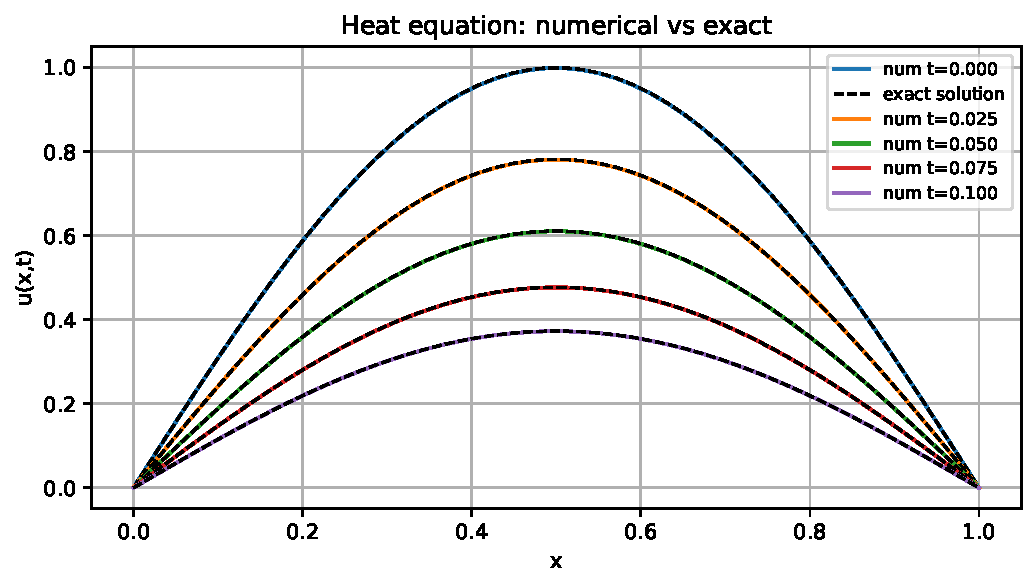
\includegraphics[keepaspectratio]{chapters/level4_finite_differences_files/figure-pdf/cell-2-output-1.pdf}}

\begin{center}\rule{0.5\linewidth}{0.5pt}\end{center}

\subsection{Remarks}\label{remarks}

\begin{itemize}
\tightlist
\item
  The \textbf{linear algebra structure} \(u^{(j+1)} = A u^{(j)} + b\)
  makes the scheme compact and systematic.\\
\item
  The stability restriction \(\lambda \leq \tfrac{1}{2}\) follows from
  analyzing the eigenvalues of \(A\).\\
\item
  For large \(N_x\), \(A\) is sparse and tridiagonal --- in practice,
  use \texttt{scipy.sparse.diags} for efficiency.
\end{itemize}

\section{Backward Difference (Implicit) Scheme for the Heat
Equation}\label{backward-difference-implicit-scheme-for-the-heat-equation}

\textbf{Pavni:} Acharya, the FTCS scheme works only if
\(\lambda \leq \tfrac{1}{2}\). Is there a method that avoids this
restriction?

\textbf{Acharya:} Yes. We can use a \textbf{backward difference in
time}, together with the same central difference in space. This gives
the \textbf{Backward Euler scheme}, which is implicit but
unconditionally stable.

\textbf{Pavni:} Implicit? What does that mean?

\textbf{Acharya:} It means that the new values \(u^{n+1}\) appear on
both sides of the equation, so we must solve a system of equations at
each time step.

\begin{center}\rule{0.5\linewidth}{0.5pt}\end{center}

\subsection{Derivation}\label{derivation}

Start from the PDE: \[
u_t = \alpha^2 u_{xx}.
\]

\begin{itemize}
\item
  Approximate the time derivative with a \textbf{backward difference}:
  \[
  u_t(x_i,t^{n+1}) \;\approx\; \frac{u_i^{\,n+1} - u_i^{\,n}}{\Delta t}.
  \]
\item
  Approximate the spatial second derivative at the new time level: \[
  u_{xx}(x_i,t^{n+1}) \;\approx\; \frac{u_{i-1}^{\,n+1} - 2u_i^{\,n+1} + u_{i+1}^{\,n+1}}{(\Delta x)^2}.
  \]
\end{itemize}

The scheme becomes: \[
\frac{u_i^{\,n+1} - u_i^{\,n}}{\Delta t} 
= \alpha^2 \,\frac{u_{i-1}^{\,n+1} - 2u_i^{\,n+1} + u_{i+1}^{\,n+1}}{(\Delta x)^2}.
\]

Rearrange: \[
- \lambda\, u_{i-1}^{\,n+1} + (1+2\lambda)\,u_i^{\,n+1} - \lambda\, u_{i+1}^{\,n+1} = u_i^{\,n},
\qquad 
\lambda = \frac{\alpha^2 \Delta t}{(\Delta x)^2}.
\]

\begin{center}\rule{0.5\linewidth}{0.5pt}\end{center}

\subsection{Matrix Form}\label{matrix-form}

Let \(u^{(n)}\) be the vector of interior values at time step \(n\).
Then \[
B u^{(n+1)} = u^{(n)},
\] where \[
B =
\begin{bmatrix}
1+2\lambda & -\lambda     &            &            &   \\
-\lambda    & 1+2\lambda  & -\lambda   &            &   \\
            & \ddots      & \ddots     & \ddots     &   \\
            &             & -\lambda   & 1+2\lambda & -\lambda \\
            &             &            & -\lambda   & 1+2\lambda
\end{bmatrix}_{(N_x-2)\times(N_x-2)}.
\]

So each step requires solving the linear system \[
u^{(n+1)} = B^{-1} u^{(n)}.
\]

\begin{center}\rule{0.5\linewidth}{0.5pt}\end{center}

\subsection{Stability}\label{stability}

\textbf{Pavni:} Doesn't that make it more expensive than FTCS?

\textbf{Acharya:} It does, because we must solve a tridiagonal system at
every time step.\\
But the reward is \textbf{unconditional stability}: for any
\(\Delta t > 0\) and \(\Delta x > 0\), the scheme does not blow up.

\textbf{Pavni:} So no restriction like \(\lambda \leq \tfrac{1}{2}\)?

\textbf{Acharya:} Exactly. Backward Euler is stable for all
\(\lambda\).\\
It is only first-order accurate in time (like FTCS), but still
second-order in space.

\begin{center}\rule{0.5\linewidth}{0.5pt}\end{center}

\subsection{Remarks}\label{remarks-1}

\begin{itemize}
\tightlist
\item
  Backward Euler is more robust but requires solving a linear system at
  each step.\\
\item
  For large systems, efficient algorithms like the \textbf{Thomas
  algorithm} (specialized Gaussian elimination for tridiagonal matrices)
  are used.\\
\item
  In practice, one balances cost (explicit FTCS, cheap but conditionally
  stable) against robustness (implicit Backward Euler, unconditionally
  stable).
\end{itemize}

\begin{tcolorbox}[enhanced jigsaw, toprule=.15mm, opacityback=0, rightrule=.15mm, breakable, colframe=quarto-callout-note-color-frame, coltitle=black, toptitle=1mm, titlerule=0mm, left=2mm, bottomrule=.15mm, leftrule=.75mm, colback=white, colbacktitle=quarto-callout-note-color!10!white, bottomtitle=1mm, opacitybacktitle=0.6, title=\textcolor{quarto-callout-note-color}{\faInfo}\hspace{0.5em}{Why the Backward Euler scheme is unconditionally stable}, arc=.35mm]

If the update is\\
\[
u^{(n+1)} = A u^{(n)},
\]\\
and the initial error is \(e^0\), then after \(n\) steps the error is\\
\[
e^{(n)} = A^n e^0.
\]

As before, the asymptotic condition is that the \textbf{spectral radius}
\(\rho(A)<1\).

\begin{center}\rule{0.5\linewidth}{0.5pt}\end{center}

\subsubsection{Eigenvalues of the Backward Euler iteration
matrix}\label{eigenvalues-of-the-backward-euler-iteration-matrix}

The Backward Euler scheme for the heat equation is\\
\[
\frac{U^{n+1} - U^n}{\Delta t} = \alpha^2 A U^{n+1},
\] which rearranges to\\
\[
U^{n+1} = (I - \lambda A)^{-1} U^n, 
\qquad \lambda = \frac{\alpha^2 \Delta t}{(\Delta x)^2}.
\]

\begin{itemize}
\item
  If \(\lambda_i(A)\) are the eigenvalues of the discrete Laplacian
  \(A\),\\
  then the eigenvalues of the iteration matrix are \[
  \mu_i = \frac{1}{1 - \lambda_i(A)}.
  \]
\item
  For the 1D Laplacian with Dirichlet BCs, \[
  \lambda_i(A) = -4 \sin^2\!\left(\frac{i\pi}{2m}\right), 
  \qquad i=1,2,\dots,m-1.
  \]
\end{itemize}

Thus \[
\mu_i = \frac{1}{1 + 4\lambda \sin^2\!\left(\frac{i\pi}{2m}\right)}.
\]

\begin{center}\rule{0.5\linewidth}{0.5pt}\end{center}

\subsubsection{Stability condition}\label{stability-condition-2}

\begin{itemize}
\tightlist
\item
  Since \(\lambda>0\) and \(\sin^2(\cdot)\ge0\),\\
  the denominator is always greater than \(1\).\\
\item
  Therefore \[
  0 < \mu_i < 1, \qquad \forall i.
  \]
\end{itemize}

This means all eigenvalues of the iteration matrix lie strictly inside
the unit circle.

\begin{center}\rule{0.5\linewidth}{0.5pt}\end{center}

✅ Thus, the \textbf{Backward Euler scheme is unconditionally stable}: -
No restriction on \(\Delta t\).\\
- Every mode decays monotonically.\\
- In contrast, FTCS required \(\lambda \le \tfrac{1}{2}\) for stability.

\end{tcolorbox}

\subsection{Interactive plots to see the eigenvalues of FTCS and
Backward Differencce
methods}\label{interactive-plots-to-see-the-eigenvalues-of-ftcs-and-backward-differencce-methods}

\begin{verbatim}
Unable to display output for mime type(s): text/html
\end{verbatim}

\begin{verbatim}
Unable to display output for mime type(s): text/html
\end{verbatim}

\begin{verbatim}
Unable to display output for mime type(s): text/html
\end{verbatim}

\begin{center}\rule{0.5\linewidth}{0.5pt}\end{center}

\textbf{How to interact with the plots} - Move the \textbf{slider} to
change \(\lambda = \tfrac{\alpha^2 \Delta t}{(\Delta x)^2}\).\\
- \textbf{FTCS plot}: notice that for \(\lambda > 0.5\) some eigenvalues
leave \([-1,1]\), indicating instability.\\
- \textbf{Backward Euler plot}: eigenvalues always remain in \((0,1)\),
showing unconditional stability.\\
- Hover over points to see their values, zoom by dragging, double-click
to reset.

\bookmarksetup{startatroot}

\chapter{Crank--Nicolson scheme}\label{cranknicolson-scheme}

\textbf{Pavni:} We've studied FTCS and Backward Euler for the heat
equation. FTCS was simple, but had that annoying stability restriction
\(\lambda \leq \tfrac{1}{2}\).

\textbf{Acharya:} Yes. And Backward Euler solved that problem --- it was
unconditionally stable.

\textbf{Pavni:} But both of them are only \emph{first-order accurate in
time}, right?

\textbf{Acharya:} Exactly. And that's a problem if we want more accuracy
without shrinking \(\Delta t\) too much.

\textbf{Pavni:} So FTCS is unstable unless
\(\lambda \leq \tfrac{1}{2}\), and Backward Euler is stable but too
diffusive. We're still missing something better.

\textbf{Acharya:} That's where the \textbf{Crank--Nicolson scheme} comes
in. The idea is to apply the trapezoidal rule in time --- using the
\emph{average} of the spatial derivative at times \(n\) and \(n+1\).

\textbf{Pavni:} So instead of evaluating only at the old time (FTCS) or
the new time (Backward Euler), we take a balance of both?

\textbf{Acharya:} Exactly. That trick makes the scheme
\textbf{second-order accurate in time} and \textbf{unconditionally
stable}. It's like combining the strengths of both FTCS and Backward
Euler.

\textbf{Pavni:} Ah, so Crank--Nicolson is really about accuracy as well
as stability. That sounds worth deriving!\\
\textbf{Pavni:} Let's derive Crank--Nicolson starting from the heat
equation \(u_t=\alpha^2 u_{xx}\). How do we get the time-centered
scheme?

\textbf{Acharya:} Start by integrating the PDE in time over one step,
from \(t^n\) to \(t^{n+1}\) at a fixed \(x\): \[
u(x,t^{n+1})-u(x,t^n)=\alpha^2\int_{t^n}^{t^{n+1}} u_{xx}(x,t)\,dt.
\]

\textbf{Pavni:} Now approximate that time integral --- I remember the
trapezoidal (averaging) rule.

\textbf{Acharya:} Exactly. Apply the trapezoidal rule to the integral on
the right: \[
\int_{t^n}^{t^{n+1}} u_{xx}(x,t)\,dt
\approx \frac{\Delta t}{2}\big(u_{xx}(x,t^n)+u_{xx}(x,t^{n+1})\big)
\] with pointwise quadrature error \(O(\Delta t^3)\) (so after division
by \(\Delta t\) the time-discretization error is \(O(\Delta t^2)\)).

\textbf{Pavni:} Then substitute that into the integrated PDE.

\textbf{Acharya:} We get \[
u(x,t^{n+1})-u(x,t^n)
= \alpha^2\frac{\Delta t}{2}\big(u_{xx}(x,t^n)+u_{xx}(x,t^{n+1})\big) + O(\Delta t^3).
\]

\textbf{Pavni:} Next we discretize \(u_{xx}\) in space with the centered
second difference.

\textbf{Acharya:} Right. At grid point \(x_j\), \[
u_{xx}(x_j,t^\ell)\approx \frac{U_{j-1}^\ell-2U_j^\ell+U_{j+1}^\ell}{(\Delta x)^2},
\] which in vector form for interior nodes is
\(\dfrac{1}{(\Delta x)^2}A U^\ell\), where \(A\) is the usual
tridiagonal Laplacian (stencil \([1,-2,1]\)).

Substituting gives (collecting interior points into \(U^n\)) \[
U^{n+1}-U^n = \frac{\alpha^2\Delta t}{2(\Delta x)^2}\big(AU^n + AU^{n+1}\big) + \text{(truncation terms)}.
\]

\textbf{Pavni:} Introduce the nondimensional parameter \(\lambda\)?

\textbf{Acharya:} Yes, set
\(\displaystyle \lambda=\frac{\alpha^2\Delta t}{(\Delta x)^2}\). Then \[
U^{n+1}-U^n = \frac{\lambda}{2}\big(AU^n + AU^{n+1}\big) + \text{(truncation terms)}.
\] Bring \(U^{n+1}\) terms to the left to obtain \[
\Big(I-\tfrac{\lambda}{2}A\Big)U^{n+1} = \Big(I+\tfrac{\lambda}{2}A\Big)U^n.
\]

Now, let's write these matrices explicitly. The left-hand side matrix is
\[
L = I-\tfrac{\lambda}{2}A =
\begin{bmatrix}
1+\lambda & -\tfrac{\lambda}{2} & 0 & \cdots & 0\\
-\tfrac{\lambda}{2} & 1+\lambda & -\tfrac{\lambda}{2} & \ddots & \vdots\\
0 & \ddots & \ddots & \ddots & 0\\
\vdots & \ddots & -\tfrac{\lambda}{2} & 1+\lambda & -\tfrac{\lambda}{2}\\
0 & \cdots & 0 & -\tfrac{\lambda}{2} & 1+\lambda
\end{bmatrix}.
\]

The right-hand side matrix is \[
R = I+\tfrac{\lambda}{2}A =
\begin{bmatrix}
1-\lambda & \tfrac{\lambda}{2} & 0 & \cdots & 0\\
\tfrac{\lambda}{2} & 1-\lambda & \tfrac{\lambda}{2} & \ddots & \vdots\\
0 & \ddots & \ddots & \ddots & 0\\
\vdots & \ddots & \tfrac{\lambda}{2} & 1-\lambda & \tfrac{\lambda}{2}\\
0 & \cdots & 0 & \tfrac{\lambda}{2} & 1-\lambda
\end{bmatrix}.
\]

So the Crank--Nicolson scheme can be written as \[
\boxed{\,L\,U^{n+1} = R\,U^n\,}.
\]

\textbf{Pavni:} Great --- and the eigenvalue form and stability follow
from the spectral map of \(A\).

\textbf{Acharya:} Right --- each eigenvalue \(\alpha_k\) of \(A\) is
mapped to \[
\mu_k=\frac{1+\tfrac{\lambda}{2}\alpha_k}{1-\tfrac{\lambda}{2}\alpha_k},
\] and substituting
\(\alpha_k=-4\sin^2\!\big(\tfrac{k\pi}{2(N+1)}\big)\) yields \[
\mu_k=\frac{1-2\lambda \sin^2\!\big(\tfrac{k\pi}{2(N+1)}\big)}
{1+2\lambda \sin^2\!\big(\tfrac{k\pi}{2(N+1)}\big)}.
\] This shows \(|\mu_k|\le1\), so CN is unconditionally stable.

\begin{tcolorbox}[enhanced jigsaw, toprule=.15mm, opacityback=0, rightrule=.15mm, breakable, colframe=quarto-callout-note-color-frame, coltitle=black, toptitle=1mm, titlerule=0mm, left=2mm, bottomrule=.15mm, leftrule=.75mm, colback=white, colbacktitle=quarto-callout-note-color!10!white, bottomtitle=1mm, opacitybacktitle=0.6, title=\textcolor{quarto-callout-note-color}{\faInfo}\hspace{0.5em}{Crank--Nicolson: derivation summary \& stability}, arc=.35mm]

\textbf{Starting point (integrated PDE):} \[
u(x,t^{n+1})-u(x,t^n)=\alpha^2\int_{t^n}^{t^{n+1}} u_{xx}(x,t)\,dt.
\]

\textbf{Trapezoidal rule (time) + centered difference (space):} \[
\int_{t^n}^{t^{n+1}} u_{xx}\,dt
\approx \frac{\Delta t}{2}\big(u_{xx}(t^n)+u_{xx}(t^{n+1})\big),
\qquad
u_{xx}(x_j,t^\ell)\approx \frac{(AU^\ell)_j}{(\Delta x)^2}.
\]

\textbf{Matrix form (with
\(\lambda=\dfrac{\alpha^2\Delta t}{(\Delta x)^2}\)):} \[
\boxed{\;\Big(I-\tfrac{\lambda}{2}A\Big)U^{n+1} = \Big(I+\tfrac{\lambda}{2}A\Big)U^n\;.}
\]

\textbf{Eigenvalues (mode-wise):} if
\(s_k=\sin\!\big(\tfrac{k\pi}{2(N+1)}\big)\) then \[
\boxed{\;\mu_k=\frac{1-2\lambda s_k^2}{1+2\lambda s_k^2}\;, \quad k=1,\dots,N. \;}
\]

\textbf{Stability check (short):} - For \(\lambda\ge0\) and
\(0\le s_k^2\le1\) the denominator \(1+2\lambda s_k^2>0\).\\
- Hence \[
|\mu_k|=\frac{|1-2\lambda s_k^2|}{1+2\lambda s_k^2}\le1,
\] and for nontrivial modes with \(\lambda>0\) strict inequality holds.

\textbf{Conclusion:} Crank--Nicolson is \textbf{unconditionally stable}
and second-order accurate in time and space (global error
\(O(\Delta t^2+\Delta x^2)\)).

\end{tcolorbox}

\begin{verbatim}
Unable to display output for mime type(s): text/html
\end{verbatim}

\textbf{How to interact:}\\
- Move the \textbf{λ} slider to vary
\(\lambda=\dfrac{\alpha^2\Delta t}{(\Delta x)^2}\).\\
- Hover on a marker to see the exact \((k,\mu_k)\).\\
- Zoom by dragging, double-click to reset.\\
\textbf{Observe:} all \(\mu_k\) satisfy \(|\mu_k|\le1\) for every
\(\lambda\ge0\), confirming unconditional stability; for small
\(\lambda\) the modes are near \(1\), for large \(\lambda\)
high-frequency modes move nearer to \(-1\) but remain bounded in
magnitude by 1.

\bookmarksetup{startatroot}

\chapter{Level 5 --- Hyperbolic PDEs}\label{level-5-hyperbolic-pdes}

\textbf{Pavni:} Acharya, we've studied the heat equation. From theory we
know that it seems to \emph{spread} information everywhere. Does every
PDE behave like that?

\textbf{Acharya:} That's a good observation, Pavni. Not every PDE
diffuses information infinitely fast like the parabolic heat equation.\\
Some equations describe situations where information or disturbances
travel at a \emph{finite speed} --- like waves or moving traffic.

\textbf{Pavni:} So these are called \emph{hyperbolic equations}?

\textbf{Acharya:} Exactly. Hyperbolic equations are the mathematical way
of describing signals or quantities that \emph{move} through a medium
rather than \emph{diffuse}.\\
For example --- a vibrating string, sound waves in air, or even cars
moving on a road.

\textbf{Pavni:} Interesting! But why are they so different from
diffusion equations like the heat equation?

\textbf{Acharya:} Because diffusion equations allow disturbances to
spread instantaneously everywhere --- a small change at one point
affects all others immediately.\\
That's called \textbf{infinite propagation speed}.\\
But hyperbolic equations restrict influence to certain \emph{paths} in
the \((x,t)\)-plane, called \textbf{characteristics}.\\
Information travels only along these paths at a finite speed.

\textbf{Pavni:} That sounds more physical. After all, signals, sound, or
cars don't move infinitely fast!

\textbf{Acharya:} Exactly. Let's begin with a simple and familiar
example --- \textbf{traffic flow}.\\
It beautifully captures the idea of \emph{conservation} and
\emph{finite-speed motion}.

\begin{center}\rule{0.5\linewidth}{0.5pt}\end{center}

\section{🚗 The Traffic Flow Model}\label{the-traffic-flow-model}

\textbf{Pavni:} So, where do we begin?

\textbf{Acharya:} Let's define some quantities.

\begin{itemize}
\tightlist
\item
  \(\rho(x,t)\): density of cars at position \(x\) and time \(t\)
  (cars/km)\\
\item
  \(v(x,t)\): average speed of cars (km/h)\\
\item
  \(q(x,t)\): flow rate --- number of cars passing a point per unit time
  (cars/hour)
\end{itemize}

\textbf{Pavni:} So \(q\) must depend on both how many cars there are and
how fast they move?

\textbf{Acharya:} Precisely. That leads us to the simple physical
relation: \[
q = \rho v.
\]

💡 Why \(q = \rho v\)?

If a small segment of road of length \(\Delta x\) contains
\(\rho \, \Delta x\) cars,\\
and each car moves with velocity \(v\), then in time \(\Delta t\) each
car covers \(v \, \Delta t\) km.\\
So, the number of cars passing a fixed point in time \(\Delta t\) is\\
\[
(\rho \, \Delta x) \cdot \frac{v \, \Delta t}{\Delta x} = \rho v \, \Delta t.
\] Dividing by \(\Delta t\) gives \(q = \rho v\).

\begin{center}\rule{0.5\linewidth}{0.5pt}\end{center}

\section{⚙️ Conservation of Cars}\label{conservation-of-cars}

\textbf{Acharya:} Now, think of a small stretch of road between \(x_1\)
and \(x_2\).\\
Cars can only leave or enter through the ends.

\[
\frac{d}{dt}\int_{x_1}^{x_2} \rho(x,t)\,dx = q(x_1,t) - q(x_2,t).
\]

\textbf{Pavni:} That looks like conservation of mass!

\textbf{Acharya:} Exactly --- just conservation of the \emph{number of
cars}.\\
The total number of cars in the interval changes only because of the
\emph{net flow} at the boundaries.

Now, let's use the \textbf{Fundamental Theorem of Calculus} to convert
this integral form into a \emph{local differential equation}.

By the Fundamental Theorem of Calculus, \[
q(x_2,t) - q(x_1,t) = \int_{x_1}^{x_2} q_x(x,t)\,dx.
\]

Substitute this into our conservation statement: \[
\frac{d}{dt}\int_{x_1}^{x_2} \rho(x,t)\,dx = -\int_{x_1}^{x_2} q_x(x,t)\,dx.
\] Assuming \(\rho\) is smooth enough to interchange differentiation and
integration: \[
\int_{x_1}^{x_2} \rho_t(x,t)\,dx = -\int_{x_1}^{x_2} q_x(x,t)\,dx.
\]

Combine both integrals: \[
\int_{x_1}^{x_2} \big[\rho_t(x,t) + q_x(x,t)\big]\,dx = 0.
\]

\textbf{Acharya:} Now, Pavni, what does this equation tell us?

\textbf{Pavni:} It says that the integral of \(\rho_t + q_x\) over
\emph{any} interval is zero.

\textbf{Acharya:} Exactly! And that can only happen if the integrand
itself is zero \emph{everywhere}.\\
Hence, we get the \textbf{local conservation law}: \[
\boxed{\rho_t + q_x = 0.}
\]

\textbf{Pavni:} So the integral form expresses the total number of cars
in a segment being conserved,\\
and this differential form expresses that conservation \emph{at every
point} on the road!

\textbf{Acharya:} Perfectly said. This is the basic \textbf{conservation
law} for one-dimensional flow.\\
Next, if we assume each car moves at a constant speed \(a\), we'll get
the \textbf{linear advection equation.}

\textbf{Pavni:} So this describes a traffic pattern moving forward
without changing its shape?

\textbf{Acharya:} Exactly. The entire profile of car density just shifts
rightward with speed \(a\).

\begin{center}\rule{0.5\linewidth}{0.5pt}\end{center}

\section{✏️ Try to Predict}\label{try-to-predict}

\textbf{Acharya:} Before solving it, can you guess how the density will
evolve if initially the density is a bump --- say, \[
\rho(x,0) = e^{-x^2}?
\]

\textbf{Pavni:} I think it will move to the right, keeping its shape.

\textbf{Acharya:} Perfect intuition. We'll now confirm this
mathematically using \textbf{characteristics} --- special curves along
which information travels.

\begin{center}\rule{0.5\linewidth}{0.5pt}\end{center}

\section{🌊 Characteristics and the Solution of the Linear Advection
Equation}\label{characteristics-and-the-solution-of-the-linear-advection-equation}

\textbf{Pavni:} Acharya, now that we have derived the equation\\
\[
\rho_t + a\rho_x = 0, \quad a > 0,
\]\\
for cars moving at constant speed, how do we actually find \(\rho(x,t)\)
from this?

\textbf{Acharya:} Excellent question. This equation may look simple, but
it contains a beautiful idea --- that \textbf{information travels along
certain paths} in the \((x,t)\)-plane. These paths are called
\emph{characteristics}.

\begin{center}\rule{0.5\linewidth}{0.5pt}\end{center}

\subsection{Deriving the Characteristic
Curves}\label{deriving-the-characteristic-curves}

\textbf{Acharya:} Let's think of \(\rho\) as a function of both \(x\)
and \(t\).\\
Suppose we move along a curve \(x = x(t)\) in the \((x,t)\)-plane.\\
By the chain rule, the total derivative of \(\rho\) along that curve is
\[
\frac{d\rho}{dt} = \rho_t + \frac{dx}{dt}\rho_x.
\]

Now, if we choose \(\dfrac{dx}{dt} = a\), then \[
\frac{d\rho}{dt} = \rho_t + a\rho_x = 0.
\]

That means \(\rho\) is \textbf{constant} along any curve that satisfies
\(\dfrac{dx}{dt} = a\).

\textbf{Pavni:} So those are the characteristic curves?

\textbf{Acharya:} Exactly! Integrating \(\dfrac{dx}{dt} = a\) gives \[
x = a t + x_0, \quad \text{or} \quad x - a t = x_0 = \text{constant}.
\]

Each line \(x - a t = \text{constant}\) is a \textbf{characteristic
line}.

\begin{center}\rule{0.5\linewidth}{0.5pt}\end{center}

\subsection{The Meaning of
Characteristics}\label{the-meaning-of-characteristics}

\textbf{Pavni:} What does it mean that \(\rho\) is constant along these
lines?

\textbf{Acharya:} It means that the value of \(\rho\) at time \(t\) and
position \(x\)\\
is exactly the same as its value at the point where that characteristic
line started on the \(x\)-axis (that is, at time \(t=0\)).

So, \[
\rho(x,t) = \rho_0(x - a t),
\] where \(\rho_0(x)\) is the initial density at \(t=0\).

\textbf{Pavni:} Oh! So the initial profile just shifts by \(a t\)?

\textbf{Acharya:} Exactly --- it moves to the right if \(a>0\) and to
the left if \(a<0\).\\
No change in shape --- pure translation.

\begin{center}\rule{0.5\linewidth}{0.5pt}\end{center}

\subsection{Verifying the Solution}\label{verifying-the-solution}

\textbf{Pavni:} Let's check if this really satisfies the PDE.

\textbf{Acharya:} Sure! Let \(\rho(x,t) = \rho_0(x - a t)\).\\
Then \[
\rho_t = -a\rho_0'(x - a t), \quad \rho_x = \rho_0'(x - a t).
\] Substitute into \(\rho_t + a\rho_x = 0\): \[
(-a\rho_0') + a\rho_0' = 0.
\] ✅ It satisfies the equation perfectly.

\begin{center}\rule{0.5\linewidth}{0.5pt}\end{center}

\subsection{Understanding Finite Propagation
Speed}\label{understanding-finite-propagation-speed}

\textbf{Acharya:} The key property of this equation is that information
moves at a \emph{finite speed}.

If a disturbance is initially present only between \(x=0\) and
\(x=1\),\\
then at time \(t\) it will be found only between \(x=a t\) and
\(x=1+a t\).\\
Every point outside this region remains unaffected.

\textbf{Pavni:} So information doesn't spread instantly like in the heat
equation?

\textbf{Acharya:} Exactly. In the \textbf{heat equation}, even a small
bump affects the whole line immediately --- infinite propagation
speed.\\
But here, the influence travels only along straight lines
\(x - a t = \text{constant}\) --- that's \textbf{finite-speed
propagation}.

\begin{center}\rule{0.5\linewidth}{0.5pt}\end{center}

\subsection{Example}\label{example}

Let's take an initial density \[
\rho_0(x) =
\begin{cases}
1, & 0 < x < 1, \\
0, & \text{otherwise}.
\end{cases}
\]

Then \[
\rho(x,t) =
\begin{cases}
1, & a t < x < 1 + a t, \\
0, & \text{otherwise}.
\end{cases}
\]

\textbf{Pavni:} So the block of cars just moves forward as a group?

\textbf{Acharya:} Exactly --- like a moving traffic wave with constant
shape.

\begin{center}\rule{0.5\linewidth}{0.5pt}\end{center}

\subsection{Visualizing
Characteristics}\label{visualizing-characteristics}

Each characteristic line shows where information travels:

\begin{Shaded}
\begin{Highlighting}[]
\NormalTok{t ↑}
\NormalTok{  |}
\NormalTok{  |       /    /    /    /    /    /    /}
\NormalTok{  |      /    /    /    /    /    /    /}
\NormalTok{  |     /    /    /    /    /    /    /}
\NormalTok{  |\_\_\_\_/\_\_\_\_/\_\_\_\_/\_\_\_\_/\_\_\_\_/\_\_\_\_/\_\_\_\_/→ x}
\end{Highlighting}
\end{Shaded}

\section{🕸️ Domain of Dependence and Domain of
Influence}\label{domain-of-dependence-and-domain-of-influence}

\textbf{Pavni:} Acharya, you mentioned earlier that information in
hyperbolic equations travels along characteristics. But how exactly do
we describe \emph{which} parts of the initial data influence the
solution at a given point?

\textbf{Acharya:} Excellent question, Pavni. To answer that, we
introduce two key ideas --- the \textbf{domain of dependence} and the
\textbf{domain of influence}. These describe how information moves
through space and time.

\begin{center}\rule{0.5\linewidth}{0.5pt}\end{center}

\subsection{What do these mean?}\label{what-do-these-mean}

\textbf{Acharya:} Let's begin intuitively.

\begin{itemize}
\item
  The \textbf{domain of dependence (DoD)} of a point \((x,t)\) is the
  set of points in the initial data that can \emph{affect} the solution
  at \((x,t)\).\\
  In other words: \emph{Which initial points influence the value here?}
\item
  The \textbf{domain of influence (DoI)} of a point \((x_0,0)\) is the
  set of space--time points \((x,t)\) that can be affected by that
  initial point.\\
  In other words: \emph{Where does the information starting at \(x_0\)
  go?}
\end{itemize}

\textbf{Pavni:} So the DoD looks backward in time, and the DoI looks
forward?

\textbf{Acharya:} Exactly. They're like mirror images of each other.\\
For hyperbolic PDEs, these regions are bounded by
\textbf{characteristics} --- the paths along which information travels
at finite speed.

\begin{center}\rule{0.5\linewidth}{0.5pt}\end{center}

\subsection{Example 1: Linear
Advection}\label{example-1-linear-advection}

\textbf{Pavni:} Let's try this with the advection equation again:\\
\[
u_t + a\,u_x = 0, \quad u(x,0) = u_0(x).
\]

\textbf{Acharya:} Good. The characteristics are the straight lines \[
x - a t = \text{constant}.
\]

So each point \((x,t)\) connects to exactly one point on the
\(x\)--axis: \(x_0 = x - a t\).

\textbf{Pavni:} So the value \(u(x,t)\) depends only on
\(u_0(x - a t)\)?

\textbf{Acharya:} Exactly. That means:

\begin{itemize}
\tightlist
\item
  The \textbf{domain of dependence} of \((x,t)\) is the \textbf{single
  point} \(x_0 = x - a t\).\\
\item
  The \textbf{domain of influence} of an initial point \((x_0,0)\) is
  the \textbf{straight line} \(x = x_0 + a t\).
\end{itemize}

\textbf{Pavni:} So for advection, both DoD and DoI are just lines ---
not regions?

\textbf{Acharya:} Right. A \emph{single characteristic line} carries all
the information.\\
This is why the advection equation has such a clean propagation behavior
--- each point of initial data simply moves at speed \(a\) without
interacting with others.

\begin{center}\rule{0.5\linewidth}{0.5pt}\end{center}

\subsection{Example 2: The 1-D Wave
Equation}\label{example-2-the-1-d-wave-equation}

\textbf{Pavni:} What happens for the wave equation?\\
\[
u_{tt} = c^2 u_{xx}.
\]

\textbf{Acharya:} Ah, this one is a bit richer. The general solution is
given by d'Alembert's formula: \[
u(x,t) = F(x - c t) + G(x + c t).
\]

\textbf{Pavni:} So now we have two families of characteristics --- one
moving right, one left?

\textbf{Acharya:} Precisely! For this equation: - Right-moving
characteristics: \(x - c t = \text{constant}\)\\
- Left-moving characteristics: \(x + c t = \text{constant}\)

Now, to find the value at \((x,t)\), you need both \(F\) and \(G\) ---
meaning information from \textbf{two points} on the initial line: \[
x - c t \quad \text{and} \quad x + c t.
\]

\textbf{Pavni:} So the DoD of \((x,t)\) is the interval between those
two points?

\textbf{Acharya:} Yes. The \textbf{domain of dependence} is\\
\[
[x - c t,\, x + c t].
\]

And the \textbf{domain of influence} of an initial point \((x_0,0)\) is
the cone-shaped region.

\pandocbounded{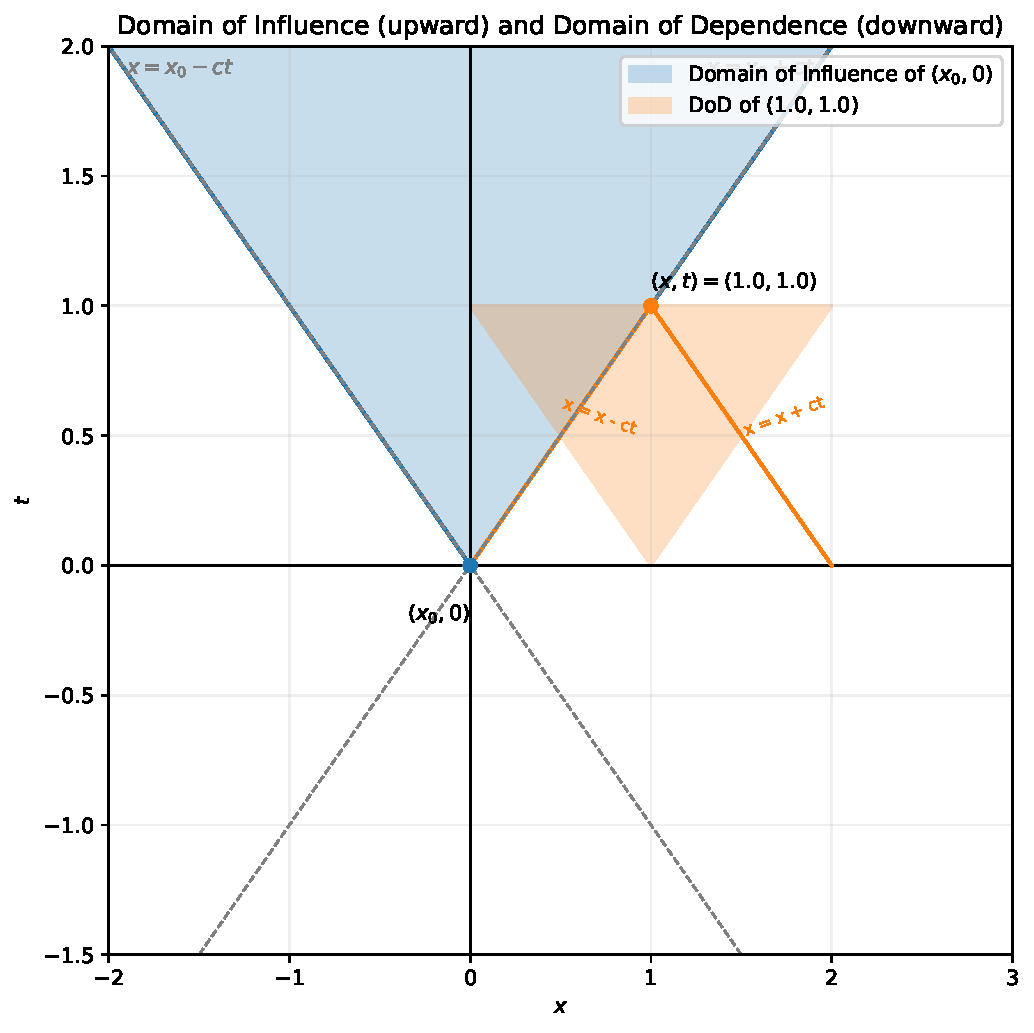
\includegraphics[keepaspectratio]{chapters/level5_Wave_Equation_files/figure-pdf/cell-2-output-1.pdf}}

\section{🚦 Nonlinear Advection and the Formation of
Shocks}\label{nonlinear-advection-and-the-formation-of-shocks}

\textbf{Pavni:} Acharya, the linear advection equation made perfect
sense --- the whole profile just moves without changing shape.\\
But traffic jams don't behave that nicely! Sometimes cars slow down
abruptly and the jam gets worse over time.\\
Does our model capture that?

\textbf{Acharya:} Excellent question, Pavni. The linear advection
equation assumes that every car moves with the \emph{same constant
speed} \(a\).\\
But in reality, cars move \textbf{slower when the road is crowded} ---
so the speed depends on the density of cars, \(\rho\).

\textbf{Pavni:} So \(v\) depends on \(\rho\)? Like \(v = v(\rho)\)?

\textbf{Acharya:} Exactly. That makes the flux \(q = \rho v(\rho)\) a
nonlinear function of \(\rho\).\\
Substituting this into the conservation law\\
\[
\rho_t + q_x = 0,
\]\\
we get the \textbf{nonlinear advection equation}: \[
\rho_t + \big(f(\rho)\big)_x = 0,
\] where \(f(\rho) = \rho v(\rho)\).

\begin{center}\rule{0.5\linewidth}{0.5pt}\end{center}

\subsection{Example: Traffic Flow
Model}\label{example-traffic-flow-model}

\textbf{Pavni:} What kind of \(v(\rho)\) should we take?

\textbf{Acharya:} A simple and realistic choice is\\
\[
v(\rho) = 1 - \rho,
\]\\
meaning cars move at unit speed when the road is empty (\(\rho=0\)),\\
and stop completely when the road is jammed (\(\rho=1\)).

Then\\
\[
f(\rho) = \rho(1 - \rho) = \rho - \rho^2,
\]\\
and our equation becomes \[
\rho_t + (\rho - \rho^2)_x = 0.
\]

\textbf{Pavni:} Expanding that gives \[
\rho_t + (1 - 2\rho)\rho_x = 0.
\] So it looks just like the advection equation, but the wave speed now
depends on \(\rho\) itself!

\textbf{Acharya:} Exactly! This is called the \textbf{nonlinear
advection equation} or \textbf{inviscid Burgers' equation}.

\begin{center}\rule{0.5\linewidth}{0.5pt}\end{center}

\section{🌀 Characteristics in the Nonlinear
Case}\label{characteristics-in-the-nonlinear-case}

\textbf{Pavni:} Earlier, for \(\rho_t + a\rho_x = 0\), we had straight
characteristic lines \(x - at = \text{constant}\).\\
How does it work here when the speed depends on \(\rho\)?

\textbf{Acharya:} Let's find out. As before, along a curve \(x = x(t)\),
the total derivative is \[
\frac{d\rho}{dt} = \rho_t + \frac{dx}{dt}\rho_x.
\] From the PDE, \[
\rho_t = -(1 - 2\rho)\rho_x.
\] Substitute this: \[
\frac{d\rho}{dt} = \rho_t + \frac{dx}{dt}\rho_x = \big[-(1 - 2\rho) + \frac{dx}{dt}\big]\rho_x.
\] For \(\dfrac{d\rho}{dt}=0\) along a characteristic, we must have \[
\frac{dx}{dt} = 1 - 2\rho.
\]

\textbf{Pavni:} So, \(\rho\) is constant along a curve whose slope
depends on \(\rho\) itself?

\textbf{Acharya:} Precisely!\\
Each ``traffic packet'' (region of constant density) moves with its own
speed \(1 - 2\rho\).\\
That's the big difference from the linear case --- now the
\textbf{characteristics themselves depend on the solution}.

\begin{center}\rule{0.5\linewidth}{0.5pt}\end{center}

\section{🚗 When Characteristics Meet --- Shock
Formation}\label{when-characteristics-meet-shock-formation}

\textbf{Pavni:} What happens if cars ahead are slower than those
behind?\\
Would the faster ones eventually catch up?

\textbf{Acharya:} That's the perfect intuition. Let's see what that
means mathematically.

Suppose initially \(\rho(x,0)\) decreases with \(x\) --- that is, higher
density (slower cars) ahead, and lower density (faster cars) behind.\\
Then the characteristic speed \(1 - 2\rho\) is \textbf{larger behind}
and \textbf{smaller ahead}.

That means characteristics \textbf{converge} --- they start to
intersect.\\
When that happens, two different characteristic lines try to assign
\emph{different values} of \(\rho\) at the same \((x,t)\).

\textbf{Pavni:} So the solution becomes \emph{multivalued}? That's not
physical.

\textbf{Acharya:} Exactly --- in reality, when cars catch up, a
\textbf{shock} forms --- a sharp front separating high and low
densities.\\
The PDE solution must then be replaced by a \emph{weak solution} that
allows for discontinuities satisfying the \textbf{Rankine--Hugoniot
condition}.

\begin{center}\rule{0.5\linewidth}{0.5pt}\end{center}

\section{⚡ The Shock Speed (Rankine--Hugoniot
Condition)}\label{the-shock-speed-rankinehugoniot-condition}

Let the shock position be \(x = s(t)\).\\
On the left of the shock, density is \(\rho_L\); on the right, it's
\(\rho_R\).

Conservation of cars gives the jump condition \[
\frac{ds}{dt} = \frac{f(\rho_L) - f(\rho_R)}{\rho_L - \rho_R}.
\]

\textbf{Pavni:} So the shock moves at a speed equal to the slope of the
line joining the two points on the flux curve \(f(\rho)\)?

\textbf{Acharya:} Perfect!\\
That's a nice geometric interpretation --- the \textbf{secant slope}
between \((\rho_L, f(\rho_L))\) and \((\rho_R, f(\rho_R))\).

For our example \(f(\rho) = \rho(1 - \rho)\), we get \[
\frac{ds}{dt} = \frac{\rho_L(1 - \rho_L) - \rho_R(1 - \rho_R)}{\rho_L - \rho_R}
              = 1 - (\rho_L + \rho_R).
\]

\begin{center}\rule{0.5\linewidth}{0.5pt}\end{center}

\section{🌊 Example: A Forming Traffic
Jam}\label{example-a-forming-traffic-jam}

\textbf{Pavni:} Let's take an example!

\textbf{Acharya:} Suppose the initial density is \[
\rho(x,0) =
\begin{cases}
0.8, & x < 0, \\
0.2, & x > 0.
\end{cases}
\]

Then \(\rho_L = 0.8\) (slow cars ahead) and \(\rho_R = 0.2\) (fast cars
behind).\\
The shock speed is \[
s' = 1 - (0.8 + 0.2) = 0.
\]

\textbf{Pavni:} So the shock doesn't move --- it stays fixed in place?

\textbf{Acharya:} Exactly! That represents a \emph{stationary traffic
jam} --- cars pile up until the density behind adjusts.\\
If we reverse the situation --- slower cars behind faster ones --- the
characteristics diverge instead, creating a \textbf{rarefaction wave}
rather than a shock.

\begin{center}\rule{0.5\linewidth}{0.5pt}\end{center}

\section{✨ Key Takeaways}\label{key-takeaways}

\begin{itemize}
\tightlist
\item
  Linear advection: constant-speed characteristics → waves move
  unchanged.\\
\item
  Nonlinear advection: speed depends on \(\rho\) → characteristics can
  intersect.\\
\item
  When they intersect, shocks form --- discontinuous but physically
  meaningful solutions.\\
\item
  The shock speed is determined by the Rankine--Hugoniot condition.\\
\item
  This mechanism underlies shock waves, traffic jams, and compressible
  fluid flows.
\end{itemize}

\begin{center}\rule{0.5\linewidth}{0.5pt}\end{center}

\textbf{Pavni:} Wow, so from traffic flow we've reached the idea of
\emph{shock waves}!\\
That's amazing --- how a simple conservation law captures such complex
behavior.

\textbf{Acharya:} That's the beauty of hyperbolic equations --- they
describe how \emph{information} and \emph{discontinuities} propagate in
nature.

\section{🚦 Shock Waves}\label{shock-waves}

\textbf{Pavni:} Acharya, we saw how nonlinear advection can either
\emph{spread out} into a rarefaction or \emph{pile up} into a shock. Can
we work through a concrete example --- step by step --- and actually
\emph{see} the shock form?

\textbf{Acharya:} Absolutely. Let's use the simple traffic-inspired
Burgers'-type model we had earlier: \[
\rho_t + (1-2\rho)\,\rho_x = 0,
\] so the characteristic speed is \[
c(\rho) = 1 - 2\rho.
\]

We will pick an initial condition that produces a shock: \[
\rho(x,0)=\begin{cases}
0.2, & x<0,\\[4pt]
0.8, & x>0.
\end{cases}
\]

\textbf{Pavni:} That's the case where the left side is sparse (fast) and
the right side is dense (slow), so I expect traffic from the left to run
into slow traffic on the right. That should make a shock, right?

\textbf{Acharya:} Exactly. Let's make the statements precise.

\begin{itemize}
\tightlist
\item
  Left state: \(\rho_L=0.2 \Rightarrow c_L = 1-2(0.2)=0.6\) (moves
  right).\\
\item
  Right state: \(\rho_R=0.8 \Rightarrow c_R = 1-2(0.8)=-0.6\) (moves
  left).
\end{itemize}

The two families of characteristics coming from left and right
\textbf{collide} --- they cross in the \((x,t)\)-plane --- so the
continuous solution breaks down and a shock forms.

\textbf{Pavni:} And the shock speed is given by the Rankine--Hugoniot
condition?

\textbf{Acharya:} Correct. For a conservation law
\(\rho_t + f(\rho)_x=0\) the shock speed \(s\) satisfies \[
s = \frac{f(\rho_L)-f(\rho_R)}{\rho_L-\rho_R}.
\] Here \(f(\rho)=\rho(1-\rho)\), so for our numbers \[
f(\rho_L)=0.2(0.8)=0.16,\qquad f(\rho_R)=0.8(0.2)=0.16,
\] hence \(s = \dfrac{0.16-0.16}{0.2-0.8}=0\).\\
So this particular shock is \emph{stationary} --- the discontinuity sits
at \(x=0\) while characteristics run into it.

\section{🚗 Interactive Exploration --- Shock vs
Rarefaction}\label{interactive-exploration-shock-vs-rarefaction}

\textbf{Acharya:} Let's play! Try changing the left and right densities
using the sliders below.\\
You'll see how the characteristics behave --- whether they
\emph{collide} (shock) or \emph{spread out} (rarefaction).

\begin{verbatim}
Unable to display output for mime type(s): text/html
\end{verbatim}

\begin{verbatim}
Unable to display output for mime type(s): text/html
\end{verbatim}

\section{🚦 A Moving Shock: When the Traffic Jam
Travels}\label{a-moving-shock-when-the-traffic-jam-travels}

\textbf{Pavni:} Acharya, earlier we saw a stationary shock where the
boundary between two traffic regions just sat still.\\
Can the shock \emph{move}?

\textbf{Acharya:} Certainly, Pavni.\\
Let's take another case:

\[
\rho(x,0) =
\begin{cases}
0.6, & x < 0,\\
0.2, & x > 0.
\end{cases}
\]

Here the left side is denser --- more cars --- while the right side is
freer.\\
Let's see what happens.

\begin{center}\rule{0.5\linewidth}{0.5pt}\end{center}

\subsection{Compute the fluxes}\label{compute-the-fluxes}

\textbf{Acharya:} Our flux function is still
\(f(\rho) = \rho(1-\rho)\).\\
So,

\[
f(0.6) = 0.24, \quad f(0.2) = 0.16.
\]

The shock speed is found from the \textbf{Rankine--Hugoniot condition}:

\[
s = \frac{f(\rho_L) - f(\rho_R)}{\rho_L - \rho_R}
= \frac{0.24 - 0.16}{0.6 - 0.2} = 0.2.
\]

\textbf{Pavni:} So the shock moves \emph{to the right} with speed 0.2?

\textbf{Acharya:} Exactly.\\
Because the flux on the left is higher, the congested region pushes into
the free region ---\\
the ``traffic jam'' moves forward!

\begin{center}\rule{0.5\linewidth}{0.5pt}\end{center}

\subsection{What happens to the
characteristics?}\label{what-happens-to-the-characteristics}

\textbf{Acharya:} Let's look at the characteristic speeds:

\[
c_L = 1 - 2\rho_L = 1 - 1.2 = -0.2, \quad
c_R = 1 - 2\rho_R = 1 - 0.4 = 0.6.
\]

So on the left, lines tilt gently left; on the right, they tilt right.\\
They intersect, and the envelope of all those intersections forms the
\textbf{shock curve}:

\[
x = s t = 0.2t.
\]

\begin{center}\rule{0.5\linewidth}{0.5pt}\end{center}

\subsection{Visualizing the moving
shock}\label{visualizing-the-moving-shock}

\begin{verbatim}
Unable to display output for mime type(s): text/html
\end{verbatim}

\begin{center}\rule{0.5\linewidth}{0.5pt}\end{center}

\bookmarksetup{startatroot}

\chapter{Von Neumann Stability
Analysis}\label{von-neumann-stability-analysis}

\textbf{Pavni:} We already checked stability for the FTCS heat solver
using the matrix (eigenvalue) approach. I want to see the Fourier-mode
(von Neumann) method --- the frequency-by-frequency picture.

\textbf{Acharya:} Sure. The von Neumann method tests how individual
sinusoidal (Fourier) modes are amplified (or damped) by a linear,
constant-coefficient finite-difference scheme. Because such schemes act
independently on each Fourier mode, we can study one mode at a time and
require every mode to be non-amplifying.

\section{Von-Neumann anlysis for the FTCS
scheme}\label{von-neumann-anlysis-for-the-ftcs-scheme}

\textbf{Acharya:} Let's start from the 1-D heat equation

\[
u_t = \alpha^2 \, u_{xx}, \qquad \alpha > 0,
\]

discretized on a uniform grid \(x_j = j\Delta x\), \(t_n = n\Delta t\)
with the explicit Forward-Time Centered-Space (FTCS) scheme

\[
u_j^{\,n+1}=u_j^{\,n}+r\big(u_{j+1}^{\,n}-2u_j^{\,n}+u_{j-1}^{\,n}\big),\qquad r:=\alpha^2 \frac{\Delta t}{\Delta x^2}.
\]

(When studying errors we set \(e_j^n = u_j^n - u(x_j,t_n)\).)

\textbf{Pavni:} Why can we assume a Fourier (sinusoidal) form for the
error?

\textbf{Acharya:} Because the scheme is linear with constant
coefficients. That means if you feed a single Fourier mode into the
linear update, it stays a Fourier mode --- only its amplitude changes.
Fourier modes form a basis for discrete periodic signals, so studying
one mode suffices.

Assume an error (or mode) of the form

\[
e_j^n = \xi^n e^{i k x_j},
\]

where \(k\) is the spatial wavenumber and \(\xi\) (the amplification
factor) is the complex number that tells how the mode's amplitude
changes per time step.

\textbf{Pavni:} Plug that into the error update.

\textbf{Acharya:} The error update mirrors the scheme:

\[
e_j^{n+1} = e_j^n + r\big(e_{j+1}^n - 2e_j^n + e_{j-1}^n\big).
\]

Substitute \(e_j^n = \xi^n e^{i k x_j}\) and
\(x_{j\pm1} = x_j \pm \Delta x\):

\[
\xi^{n+1} e^{i k x_j} = \xi^n e^{i k x_j} + r\xi^n\big(e^{i k (x_j+\Delta x)} - 2 e^{i k x_j} + e^{i k (x_j-\Delta x)}\big).
\]

Cancel the common nonzero factor \(\xi^n e^{i k x_j}\) to get

\[
\xi = 1 + r\big(e^{i k \Delta x} - 2 + e^{-i k \Delta x}\big).
\]

Use \(e^{i\theta}+e^{-i\theta}=2\cos\theta\) and simplify:

\[
\xi = 1 + 2r(\cos(k\Delta x)-1) = 1 - 4r\sin^2\!\left(\frac{k\Delta x}{2}\right).
\]

This is the amplification factor for a Fourier mode of wavenumber \(k\).

\section{Stability condition}\label{stability-condition-3}

\textbf{Pavni:} So what condition on \(r\) ensures stability?

\textbf{Acharya:} For stability we require that every Fourier mode is
not amplified, i.e.

\[
|\xi| \le 1 \quad\text{for all allowed } k.
\]

For this FTCS case \(\xi\) is real, so the requirement reduces to
\(-1 \le \xi \le 1\). The maximum value of \(\xi\) is \(1\) (when
\(\sin^2=0\)), so we only need to check the minimum. The minimum occurs
when \(\sin^2(\cdot)=1\), giving \(\xi_{\min}=1-4r\). Requiring
\(\xi_{\min}\ge-1\) gives

\[
1-4r \ge -1 \quad\Longrightarrow\quad r \le \tfrac12.
\]

Hence the von Neumann stability condition is

\[
\boxed{\qquad \alpha\frac{\Delta t}{\Delta x^2} \le \tfrac12 \quad\Longleftrightarrow\quad \Delta t \le \frac{\Delta x^2}{2\alpha}\,.}
\]

\section{Comments and interpretation}\label{comments-and-interpretation}

\begin{itemize}
\tightlist
\item
  Long (low-frequency) modes have \(\sin^2\!\approx (k\Delta x/2)^2\)
  and so \(\xi\) is near \(1\); they decay slowly.\\
\item
  Short (high-frequency) modes have \(\sin^2\) near \(1\) and so are
  damped more strongly (smaller \(\xi\)).\\
\item
  If \(r>1/2\) then the shortest modes have \(\xi<-1\) leading to
  oscillatory growth and instability.\\
\item
  The von Neumann method is equivalent to the matrix/eigenvalue analysis
  for linear constant-coefficient schemes on periodic grids. Fourier
  modes are eigenvectors of circulant matrices; \(\xi(k)\) are the
  eigenvalues.
\end{itemize}

\bookmarksetup{startatroot}

\chapter{Quick exercise}\label{quick-exercise}

\begin{quote}
\textbf{Exercise.} For the heat equation FTCS scheme above, compute
\(\xi(k)\) for the two extreme wavenumbers on a grid with \(N\) points
and periodic boundary conditions: \(k=0\) and the Nyquist mode
\(k=\pi/\Delta x\). Interpret the values.
\end{quote}

Click to reveal the answer

\textbf{Answer (sketch).}\\
For \(k=0\), \(\sin^2(0)=0\) so \(\xi=1\) (constant mode preserved).\\
For \(k=\pi/\Delta x\), \(\sin^2(\pi/2)=1\) so \(\xi=1-4r\) (the maximal
damping; needs \(r\le 1/2\) to avoid instability).

\bookmarksetup{startatroot}

\chapter{Von Neumann analysis for the Upwind and Lax--Friedrichs
schemes}\label{von-neumann-analysis-for-the-upwind-and-laxfriedrichs-schemes}

\textbf{Pavni:} Now that we finished the heat equation, can we do von
Neumann analysis for a \emph{hyperbolic} equation --- say, the linear
advection equation?

\textbf{Acharya:} Perfect next step. Let's take the simplest hyperbolic
PDE:

\[
u_t + a\,u_x = 0, \qquad a>0.
\]

The exact solution is a wave that just travels to the right at speed (a)
without changing shape.

\begin{center}\rule{0.5\linewidth}{0.5pt}\end{center}

\section{1. Upwind scheme}\label{upwind-scheme}

\textbf{Pavni:} Remind me of the upwind finite difference scheme?

\textbf{Acharya:} For (a\textgreater0), we use the backward spatial
difference:

\[
u_j^{n+1} = u_j^n - C (u_j^n - u_{j-1}^n),
\]

where (C = a \frac{\Delta t}{\Delta x}) is the \textbf{Courant number}.

\begin{center}\rule{0.5\linewidth}{0.5pt}\end{center}

\subsection{Step 1 --- Assume a Fourier
mode}\label{step-1-assume-a-fourier-mode}

As before, let the error (or a representative mode) be

\[
e_j^n = \xi^n e^{i k x_j}.
\]

Substitute this into the scheme:

\[
\xi^{n+1} e^{i k x_j}
= \xi^n e^{i k x_j} - C \xi^n \big(e^{i k x_j} - e^{i k (x_j - \Delta x)}\big).
\]

Cancel the common factor ( \xi\^{}n e\^{}\{i k x\_j\}):

\[
\xi = 1 - C(1 - e^{-i k \Delta x}).
\]

Simplify using Euler's formula (e\^{}\{-i\theta\} = \cos\theta -
i\sin\theta):

\[
\boxed{\displaystyle
\xi = 1 - C(1 - \cos(k\Delta x) + i\sin(k\Delta x)).
}
\]

\begin{center}\rule{0.5\linewidth}{0.5pt}\end{center}

\subsection{\texorpdfstring{Step 2 --- Compute
\(|\xi|\)}{Step 2 --- Compute \textbar\textbackslash xi\textbar{}}}\label{step-2-compute-xi}

We need ( \textbar{}\xi\textbar{} \le 1 ) for stability.

Compute the magnitude squared:

\[
|\xi|^2 = [1 - C(1 - \cos(k\Delta x))]^2 + [C\sin(k\Delta x)]^2.
\]

Simplify a bit:

\[
|\xi|^2 = 1 - 2C(1 - \cos(k\Delta x)) + C^2( (1 - \cos(k\Delta x))^2 + \sin^2(k\Delta x)).
\]

But ( (1-\cos\theta)\^{}2 + \sin\^{}2\theta = 2(1 - \cos\theta) ).\\
Hence,

\[
|\xi|^2 = 1 - 2C(1 - \cos(k\Delta x)) + 2C^2(1 - \cos(k\Delta x)).
\]

Simplify further:

\[
|\xi|^2 = 1 - 2C(1-C)(1 - \cos(k\Delta x)).
\]

\begin{center}\rule{0.5\linewidth}{0.5pt}\end{center}

\subsection{Step 3 --- Stability
condition}\label{step-3-stability-condition}

Because (1 - \cos(k\Delta x) \ge 0), the worst case is when this factor
is maximum, i.e.~(k\Delta x = \pi).\\
So the scheme is stable if

\[
|\xi|^2 \le 1 \quad \Rightarrow \quad 2C(1-C) \ge 0.
\]

This requires (0 \le C \le 1.)

✅ \textbf{Stability condition for upwind scheme:}

\[
\boxed{\displaystyle 0 \le a\frac{\Delta t}{\Delta x} \le 1.}
\]

\begin{center}\rule{0.5\linewidth}{0.5pt}\end{center}

\textbf{Pavni:} That's the well-known CFL condition!\\
But does \(\xi\) have a complex part? So will the amplitude decay?

\textbf{Acharya:} Yes --- for \(0 < C < 1\), \(\xi\) has a nonzero
imaginary part (phase) and a real part less than 1, meaning the wave
both \emph{advects} and \emph{damps}.\\
So upwind is \textbf{stable but diffusive} --- short waves decay faster.

\begin{center}\rule{0.5\linewidth}{0.5pt}\end{center}

\section{2. Lax--Friedrichs scheme}\label{laxfriedrichs-scheme}

\textbf{Pavni:} What about the Lax--Friedrichs scheme?

\textbf{Acharya:} It's another explicit method for the same advection
equation:

\[
u_j^{n+1} = \frac{1}{2}(u_{j+1}^n + u_{j-1}^n) - \frac{C}{2}(u_{j+1}^n - u_{j-1}^n),
\]

with the same Courant number ( C = a \frac{\Delta t}{\Delta x} ).

\begin{center}\rule{0.5\linewidth}{0.5pt}\end{center}

\subsection{Step 1 --- Substitute Fourier
mode}\label{step-1-substitute-fourier-mode}

Let ( e\_j\^{}n = \xi\^{}n e\^{}\{i k x\_j\} ). Substitute into the
scheme:

\[
\xi^{n+1} e^{i k x_j}
= \frac{1}{2}\xi^n (e^{i k (x_j + \Delta x)} + e^{i k (x_j - \Delta x)}) - \frac{C}{2}\xi^n (e^{i k (x_j + \Delta x)} - e^{i k (x_j - \Delta x)}).
\]

Cancel ( \xi\^{}n e\^{}\{i k x\_j\} ):

\[
\xi = \frac{1}{2}(e^{i k \Delta x} + e^{-i k \Delta x}) - \frac{C}{2}(e^{i k \Delta x} - e^{-i k \Delta x}).
\]

Simplify using trig identities:

\[
\xi = \cos(k\Delta x) - i C \sin(k\Delta x).
\]

\begin{center}\rule{0.5\linewidth}{0.5pt}\end{center}

\subsection{Step 2 --- Magnitude
condition}\label{step-2-magnitude-condition}

Compute

\[
|\xi|^2 = \cos^2(k\Delta x) + C^2\sin^2(k\Delta x)
= 1 - (1 - C^2)\sin^2(k\Delta x).
\]

For stability, require ( \textbar{}\xi\textbar{} \le 1 ), i.e.~(
\textbar{}\xi\textbar\^{}2 \le 1 ).\\
This holds for all \(k\) \textbf{if and only if} ( \textbar C\textbar{}
\le 1. )

✅ \textbf{Stability condition for Lax--Friedrichs:}

\[
\boxed{|a|\frac{\Delta t}{\Delta x} \le 1.}
\]

\begin{center}\rule{0.5\linewidth}{0.5pt}\end{center}

\subsection{Step 3 --- Interpretation}\label{step-3-interpretation}

\textbf{Pavni:} The condition is the same as for upwind. But the form of
\(\xi\) is different.

\textbf{Acharya:} Exactly.\\
- The magnitude \(|\xi| < 1\) for all nonzero \(k\) → the scheme has
\textbf{numerical dissipation} (damps all waves).\\
- The imaginary part causes a \textbf{phase error} --- the wave travels
slightly slower than it should.\\
- As \(C \to 1\), the scheme becomes less diffusive but still stable.

\begin{center}\rule{0.5\linewidth}{0.5pt}\end{center}

Optional check: Derive \(|\xi|^2\) for both schemes and compare their
dissipation.

For small \(k\Delta x\), expand \(\sin\) and \(\cos\) to second order.\\
You'll find: - \textbf{Upwind:} amplitude decays like
\(e^{-(1-C)(k\Delta x)^2/2}\) (first-order diffusive error).\\
- \textbf{Lax--Friedrichs:} decays like \(e^{-(1-C^2)(k\Delta x)^2/2}\)
(more diffusive).

Hence, Lax--Friedrichs is more smoothing --- it damps short waves more
strongly than upwind.

\begin{center}\rule{0.5\linewidth}{0.5pt}\end{center}

\textbf{Pavni:} So both methods are stable under the CFL condition
\(|C|\le1\), but upwind is less diffusive.

\textbf{Acharya:} Right. That's why upwind is preferred for
advection-dominated problems.\\
Von Neumann analysis clearly shows the trade-off between
\textbf{stability, dissipation, and dispersion}.

\begin{center}\rule{0.5\linewidth}{0.5pt}\end{center}


\backmatter


\end{document}
